%  LaTeX support: latex@mdpi.com 
%  For support, please attach all files needed for compiling as well as the log file, and specify your operating system, LaTeX version, and LaTeX editor.

%=================================================================
\documentclass[energies,article,accept,pdftex,moreauthors]{Definitions/mdpi} 
% For posting an early version of this manuscript as a preprint, you may use "preprints" as the journal and change "submit" to "accept". The document class line would be, e.g., \documentclass[preprints,article,accept,moreauthors,pdftex]{mdpi}. This is especially recommended for submission to arXiv, where line numbers should be removed before posting. For preprints.org, the editorial staff will make this change immediately prior to posting.

%--------------------
% Class Options:
%--------------------
%----------
% journal
%----------
% Choose between the following MDPI journals:
% acoustics, actuators, addictions, admsci, adolescents, aerospace, agriculture, agriengineering, agronomy, ai, algorithms, allergies, alloys, analytica, animals, antibiotics, antibodies, antioxidants, applbiosci, appliedchem, appliedmath, applmech, applmicrobiol, applnano, applsci, aquacj, architecture, arts, asc, asi, astronomy, atmosphere, atoms, audiolres, automation, axioms, bacteria, batteries, bdcc, behavsci, beverages, biochem, bioengineering, biologics, biology, biomass, biomechanics, biomed, biomedicines, biomedinformatics, biomimetics, biomolecules, biophysica, biosensors, biotech, birds, bloods, blsf, brainsci, breath, buildings, businesses, cancers, carbon, cardiogenetics, catalysts, cells, ceramics, challenges, chemengineering, chemistry, chemosensors, chemproc, children, chips, cimb, civileng, cleantechnol, climate, clinpract, clockssleep, cmd, coasts, coatings, colloids, colorants, commodities, compounds, computation, computers, condensedmatter, conservation, constrmater, cosmetics, covid, crops, cryptography, crystals, csmf, ctn, curroncol, currophthalmol, cyber, dairy, data, dentistry, dermato, dermatopathology, designs, diabetology, diagnostics, dietetics, digital, disabilities, diseases, diversity, dna, drones, dynamics, earth, ebj, ecologies, econometrics, economies, education, ejihpe, electricity, electrochem, electronicmat, electronics, encyclopedia, endocrines, energies, eng, engproc, ent, entomology, entropy, environments, environsciproc, epidemiologia, epigenomes, est, fermentation, fibers, fintech, fire, fishes, fluids, foods, forecasting, forensicsci, forests, foundations, fractalfract, fuels, futureinternet, futureparasites, futurepharmacol, futurephys, futuretransp, galaxies, games, gases, gastroent, gastrointestdisord, gels, genealogy, genes, geographies, geohazards, geomatics, geosciences, geotechnics, geriatrics, hazardousmatters, healthcare, hearts, hemato, heritage, highthroughput, histories, horticulturae, humanities, humans, hydrobiology, hydrogen, hydrology, hygiene, idr, ijerph, ijfs, ijgi, ijms, ijns, ijtm, ijtpp, immuno, informatics, information, infrastructures, inorganics, insects, instruments, inventions, iot, j, jal, jcdd, jcm, jcp, jcs, jdb, jeta, jfb, jfmk, jimaging, jintelligence, jlpea, jmmp, jmp, jmse, jne, jnt, jof, joitmc, jor, journalmedia, jox, jpm, jrfm, jsan, jtaer, jzbg, kidney, kidneydial, knowledge, land, languages, laws, life, liquids, literature, livers, logics, logistics, lubricants, lymphatics, machines, macromol, magnetism, magnetochemistry, make, marinedrugs, materials, materproc, mathematics, mca, measurements, medicina, medicines, medsci, membranes, merits, metabolites, metals, meteorology, methane, metrology, micro, microarrays, microbiolres, micromachines, microorganisms, microplastics, minerals, mining, modelling, molbank, molecules, mps, msf, mti, muscles, nanoenergyadv, nanomanufacturing, nanomaterials, ncrna, network, neuroglia, neurolint, neurosci, nitrogen, notspecified, nri, nursrep, nutraceuticals, nutrients, obesities, oceans, ohbm, onco, oncopathology, optics, oral, organics, organoids, osteology, oxygen, parasites, parasitologia, particles, pathogens, pathophysiology, pediatrrep, pharmaceuticals, pharmaceutics, pharmacoepidemiology, pharmacy, philosophies, photochem, photonics, phycology, physchem, physics, physiologia, plants, plasma, pollutants, polymers, polysaccharides, poultry, powders, preprints, proceedings, processes, prosthesis, proteomes, psf, psych, psychiatryint, psychoactives, publications, quantumrep, quaternary, qubs, radiation, reactions, recycling, regeneration, religions, remotesensing, reports, reprodmed, resources, rheumato, risks, robotics, ruminants, safety, sci, scipharm, seeds, sensors, separations, sexes, signals, sinusitis, skins, smartcities, sna, societies, socsci, software, soilsystems, solar, solids, sports, standards, stats, stresses, surfaces, surgeries, suschem, sustainability, symmetry, synbio, systems, taxonomy, technologies, telecom, test, textiles, thalassrep, thermo, tomography, tourismhosp, toxics, toxins, transplantology, transportation, traumacare, traumas, tropicalmed, universe, urbansci, uro, vaccines, vehicles, venereology, vetsci, vibration, viruses, vision, waste, water, wem, wevj, wind, women, world, youth, zoonoticdis 

%---------
% article
%---------
% The default type of manuscript is "article", but can be replaced by: 
% abstract, addendum, article, book, bookreview, briefreport, casereport, comment, commentary, communication, conferenceproceedings, correction, conferencereport, entry, expressionofconcern, extendedabstract, datadescriptor, editorial, essay, erratum, hypothesis, interestingimage, obituary, opinion, projectreport, reply, retraction, review, perspective, protocol, shortnote, studyprotocol, systematicreview, supfile, technicalnote, viewpoint, guidelines, registeredreport, tutorial
% supfile = supplementary materials

%----------
% submit
%----------
% The class option "submit" will be changed to "accept" by the Editorial Office when the paper is accepted. This will only make changes to the frontpage (e.g., the logo of the journal will get visible), the headings, and the copyright information. Also, line numbering will be removed. Journal info and pagination for accepted papers will also be assigned by the Editorial Office.

%------------------
% moreauthors
%------------------
% If there is only one author the class option oneauthor should be used. Otherwise use the class option moreauthors.

%---------
% pdftex
%---------
% The option pdftex is for use with pdfLaTeX. If eps figures are used, remove the option pdftex and use LaTeX and dvi2pdf.
%=================================================================
% MDPI internal commands
\firstpage{1} 
\makeatletter 
\setcounter{page}{\@firstpage} 
\makeatother
\pubvolume{1}
\issuenum{1}
\articlenumber{0}
\pubyear{2023}
\copyrightyear{2023}
\externaleditor{Academic Editor: José Luís Sousa, Luís Pires Neves and António Gomes Martins}
\datereceived{3 November 2022} 
\daterevised{1 February 2023} % Only for the journal Acoustics
\dateaccepted{7 February 2023} 
\datepublished{} 
%\datecorrected{} % Corrected papers include a "Corrected: XXX" date in the original paper.
%\dateretracted{} % Corrected papers include a "Retracted: XXX" date in the original paper.
\hreflink{https://doi.org/10.3390/xxxxx} % If needed use \linebreak
%\doinum{}
%------------------------------------------------------------------
% The following line should be uncommented if the LaTeX file is uploaded to arXiv.org
%\pdfoutput=1

%=================================================================
% Add packages and commands here. The following packages are loaded in our class file: fontenc, inputenc, calc, indentfirst, fancyhdr, graphicx, epstopdf, lastpage, ifthen, lineno, float, amsmath, setspace, enumitem, mathpazo, booktabs, titlesec, etoolbox, tabto, xcolor, soul, multirow, microtype, tikz, totcount, changepage, attrib, upgreek, cleveref, amsthm, hyphenat, natbib, hyperref, footmisc, url, geometry, newfloat, caption

%=================================================================
%% Please use the following mathematics environments: Theorem, Lemma, Corollary, Proposition, Characterization, Property, Problem, Example, ExamplesandDefinitions, Hypothesis, Remark, Definition, Notation, Assumption
%% For proofs, please use the proof environment (the amsthm package is loaded by the MDPI class).

%=================================================================
% Full title of the paper (Capitalized)
\Title{Modelling Energy Data in a Generalized Additive Model---A Case Study of Colombia}

% MDPI internal command: Title for citation in the left column
\TitleCitation{Modelling Energy Data in a Generalized Additive Model---A Case Study of Colombia}

% Author Orchid ID: enter ID or remove command
%\newcommand{\orcidauthorA}{0000-0000-0000-000X} % Add \orcidA{} behind the author's name
%\newcommand{\orcidauthorB}{0000-0000-0000-000X} % Add \orcidB{} behind the author's name

% Authors, for the paper (add full first names)
\Author{Lina %MDPI: Please carefully check the accuracy of names and affiliations.
 Berbesi and Dr.Geoffrey Pritchard *} %Lina: Citation should be Dr.Geoffrey Pritchard

%\longauthorlist{yes}

% MDPI internal command: Authors, for metadata in PDF
\AuthorNames{Lina Berbesi and Dr.Geoffrey Pritchard} %Lina: Citation should be Dr.Geoffrey Pritchard

% MDPI internal command: Authors, for citation in the left column
\AuthorCitation{Berbesi%MDPI: Please carefully check the accuracy of names and affiliations.
, L.; Pritchard, G.} %%MDPI: Please add the detailed address information (city, post code and country)
% If this is a Chicago style journal: Lastname, Firstname, Firstname Lastname, and Firstname Lastname.

% Affiliations / Addresses (Add [1] after \address if there is only one affiliation.)
\address{ \quad{Department of Statistics, Faculty of Science, University of Auckland, Auckland 1010, New Zealand}
; lber562@aucklanduni.com} %Lina: I changed to Auckland university because that is where the research was conducted. It was not related with Stats New Zealand which is where I am currently working. I also changed my mail to the Auckland Uni one.

% Contact information of the corresponding author
\corres{Correspondence:  g.pritchard@auckland.ac.nz}

%\simplesumm{} % Simple summary

%\conference{} % An extended version of a conference paper

% Abstract (Do not insert blank lines, i.e., \\) %Lina: I changed the abstract to improved the flow after proof-reading with native speakers
\abstract{Energy demand modelling is essential for reliable informing and framing energy policy decisions. More accurate modelling betters ensuring availability of energy and energy quality. Energy availability is related to energy access across the country and defines important economic measures such as energy poverty, which plays a critical role in developing countries. Energy quality is related to the reliability of the supply for correctly estimating energy needs. To incorporate spatial and temporal components of energy in a way that availability and quality are accurately assessed, this article discussed a number of suitable task methods for this (Second-generation GAMs with one-dimensional smoothers: Cyclic/Non-Cyclic Cubic Splines and two-dimensional smoothers: Markov Random Fields/Tensor Splines Interactions). The results showed that the complete consideration of both temporal and spatial aspects leads to a better fitted model which explains more of the data~variation.}

%Lina's Changes: the energy needs --> energy needs (article non-required)


% Keywords
\keyword{generalized additive models; cubic splines; Markov random fields; tensor product splines; energy modelling} 

% The fields PACS, MSC, and JEL may be left empty or commented out if not applicable
%\PACS{J0101}
%\MSC{}
%\JEL{}

%%%%%%%%%%%%%%%%%%%%%%%%%%%%%%%%%%%%%%%%%%
% Only for the journal Diversity
%\LSID{\url{http://}}

%%%%%%%%%%%%%%%%%%%%%%%%%%%%%%%%%%%%%%%%%%
% Only for the journal Applied Sciences
%\featuredapplication{Authors are encouraged to provide a concise description of the specific application or a potential application of the work. This section is not mandatory.}
%%%%%%%%%%%%%%%%%%%%%%%%%%%%%%%%%%%%%%%%%%

%%%%%%%%%%%%%%%%%%%%%%%%%%%%%%%%%%%%%%%%%%
% Only for the journal Data
%\dataset{DOI number or link to the deposited data set if the data set is published separately. If the data set shall be published as a supplement to this paper, this field will be filled by the journal editors. In this case, please submit the data set as a supplement.}
%\datasetlicense{License under which the data set is made available (CC0, CC-BY, CC-BY-SA, CC-BY-NC, etc.)}

%%%%%%%%%%%%%%%%%%%%%%%%%%%%%%%%%%%%%%%%%%
% Only for the journal Toxins
%\keycontribution{The breakthroughs or highlights of the manuscript. Authors can write one or two sentences to describe the most important part of the paper.}

%%%%%%%%%%%%%%%%%%%%%%%%%%%%%%%%%%%%%%%%%%
% Only for the journal Encyclopedia
%\encyclopediadef{For entry manuscripts only: please provide a brief overview of the entry title instead of an abstract.}

%%%%%%%%%%%%%%%%%%%%%%%%%%%%%%%%%%%%%%%%%%
% Only for the journal Advances in Respiratory Medicine
%\addhighlights{yes}
%\renewcommand{\addhighlights}{%

%\noindent This is an obligatory section in “Advances in Respiratory Medicine”, whose goal is to increase the discoverability and readability of the article via search engines and other scholars. Highlights should not be a copy of the abstract, but a simple text allowing the reader to quickly and simplified find out what the article is about and what can be cited from it. Each of these parts should be devoted up to 2~bullet points.\vspace{3pt}\\
%\textbf{What are the main findings?}
% \begin{itemize}[labelsep=2.5mm,topsep=-3pt]
% \item First bullet.
% \item Second bullet.
% \end{itemize}\vspace{3pt}
%\textbf{What is the implication of the main finding?}
% \begin{itemize}[labelsep=2.5mm,topsep=-3pt]
% \item First bullet.
% \item Second bullet.
% \end{itemize}
%}

%%%%%%%%%%%%%%%%%%%%%%%%%%%%%%%%%%%%%%%%%%
\begin{document}

%%%%%%%%%%%%%%%%%%%%%%%%%%%%%%%%%%%%%%%%%%

\section{Introduction}

%Lina's changes: Electricity modelling --> Energy demand modelling (To be consistent about the fact we are talking about energy demand in the article)
%Lina's changes: they allow the identification of gaps --> they enable the identification of gaps 
%Lina's changes: which helps avoid shortages related to underestimation and avoid costs related to~overestimation --> avoiding underestimation-shortage and overestimation-costs

Energy demand modelling in developing countries plays a huge role in framing policy decisions for energy management,  as a country's rapid pace of transformation calls for models that both adjust to short-term needs but also  for more refined approaches that allow to make long-term plans for energy coverage.  In~that sense, quantitative analyses that evaluate a country's population energy consumption across time and space are important because they enable the identification of gaps in energy access and patterns in energy consumption avoiding underestimation-shortage and overestimation-costs.

%Lina's changes: Removed the specific extend of the country due to it is not necessary to know the specific extend 
Ensuring access to affordable, reliable, sustainable, and~modern energy is the seventh goal in the sustainable development goals from the United Nations~\citep{UnitedNations2018AFFORDABLEEfficient}. Unfortunately, this has been hard to accomplish for Colombia due to the geography of the country with a considerable amount of land, around a million square kilometers, equivalent to three medium-sized European countries. In addition to, natural barriers such as mountains or rivers create connectivity difficulties and lead to elevated costs of energy installations~\citep{BustosGonzalez2014NonPerspectives}. 

%Lina's changed: Moved references towards the end of the phrase

The vulnerability of the poor is aggravated by climate change and the volatility of energy prices \citep{WHO2009TheCountries} . For~tropical countries such as Colombia, those two aspects are strongly associated with temporal demand variation. On~one side, climate change makes the rainy/dry season more pronounced and aggressive, which can be addressed in a model by including a yearly pattern. On~the other side, the~volatility of energy prices is hard to control if no modelling is implemented over energy data and if the tendencies and patterns are~unknown. \clearpage

 Often the spatial aspect  is ignored when modelling energy~\citep{Meier2019Short-termModels}, meaning that  neither consulting companies nor governmental entities, especially in developing countries, include spatial  elements  in energy modelling. Nonetheless, the~spatial characteristics of the data when modelled can explain a lot about what is happening in the regions and can often be  linked to socio-economic characteristics (i.e., size or number of households) of the regions. Analyses using global data sets or global analyses often fail to provide sufficient information on energy~access \citep{WHO2009TheCountries}. % please verify Lina: That is correct I moved the reference towards the end
 
 %Lina's changes: Currenty --> TO Date

 To date, the spatial information in Colombia that is publicly accessible in regards to energy is given by the energy operators, which can be associated with regions, but there is not further detail available publicly related to households. Each energy operator has its separate household information, but this information is being sent already aggregated to the government entities that foresee the energy market. Therefore, there is no way of desegregating the data at a further level of~detail. 

%Lina's changes: Moved references towards the end
%Lina's changes: Changed the percentages to words according to APA's rules/ Also changed the numbers to words
%Lina's changes: has addressed - addresses
%Lina's changes: I split the 2014 sentence in two because it was too long and removed the names of the regions because you can inferred that information from Figure 1

In 2007, four percent of the Colombian population was not connected to the national grid accounting for sixty-six percent of the national territory \citep{Franco2007ContributionSouthwest}. Since then there has not been any other publication that addresses the percentage of the population that dwells in the non interconnected energy grid areas,  this could nevertheless be inferred from the reports of non-interconnected zones/departments plus census data. In 2014 a map of non-interconnected zones showed that eleven out of the thirty-two departments were partially or entirely not connected to the grid\citep{BustosGonzalez2014NonPerspectives} (See figure ~\ref{fig:1}). This is equivalent to fifty-four percent of the territory when measured by department area. An analysis over historical demand in 2018 unveiled that five out of thirty-two departments were not connected to the national grid which is equivalent to thirty percent of the territory when measured by department~area ~\citep{XMHistoricalDemand}. Even with an improvement of twenty percent on energy coverage between the years 2014 and 2018 there is still a significant portion of the country that is not being accounted for.

%Lina's changes: Removing which 
Scarcity in energy access or availability is common in developing countries, inherently related to space rather than time makes modelling exclusively with temporal parameters not ideal. Broadening the access to modern energy services is something that needs to be addressed by all countries but also represents a colossal challenge for the developing ones ~\citep{WHO2009TheCountries}. 

%Lina's changes: I removed main~contributions bullet points and summarize them in a paragraph

This article explores the potential of combining spatial and temporal data for improving the reliability of energy demand modelling in Colombia with the constraints data available to date has while stating modelling possibilities for future data desegregated at a lower level.


      \begin{figure}[H]
	%\centering
	%\hspace{-1em}
   \centering
		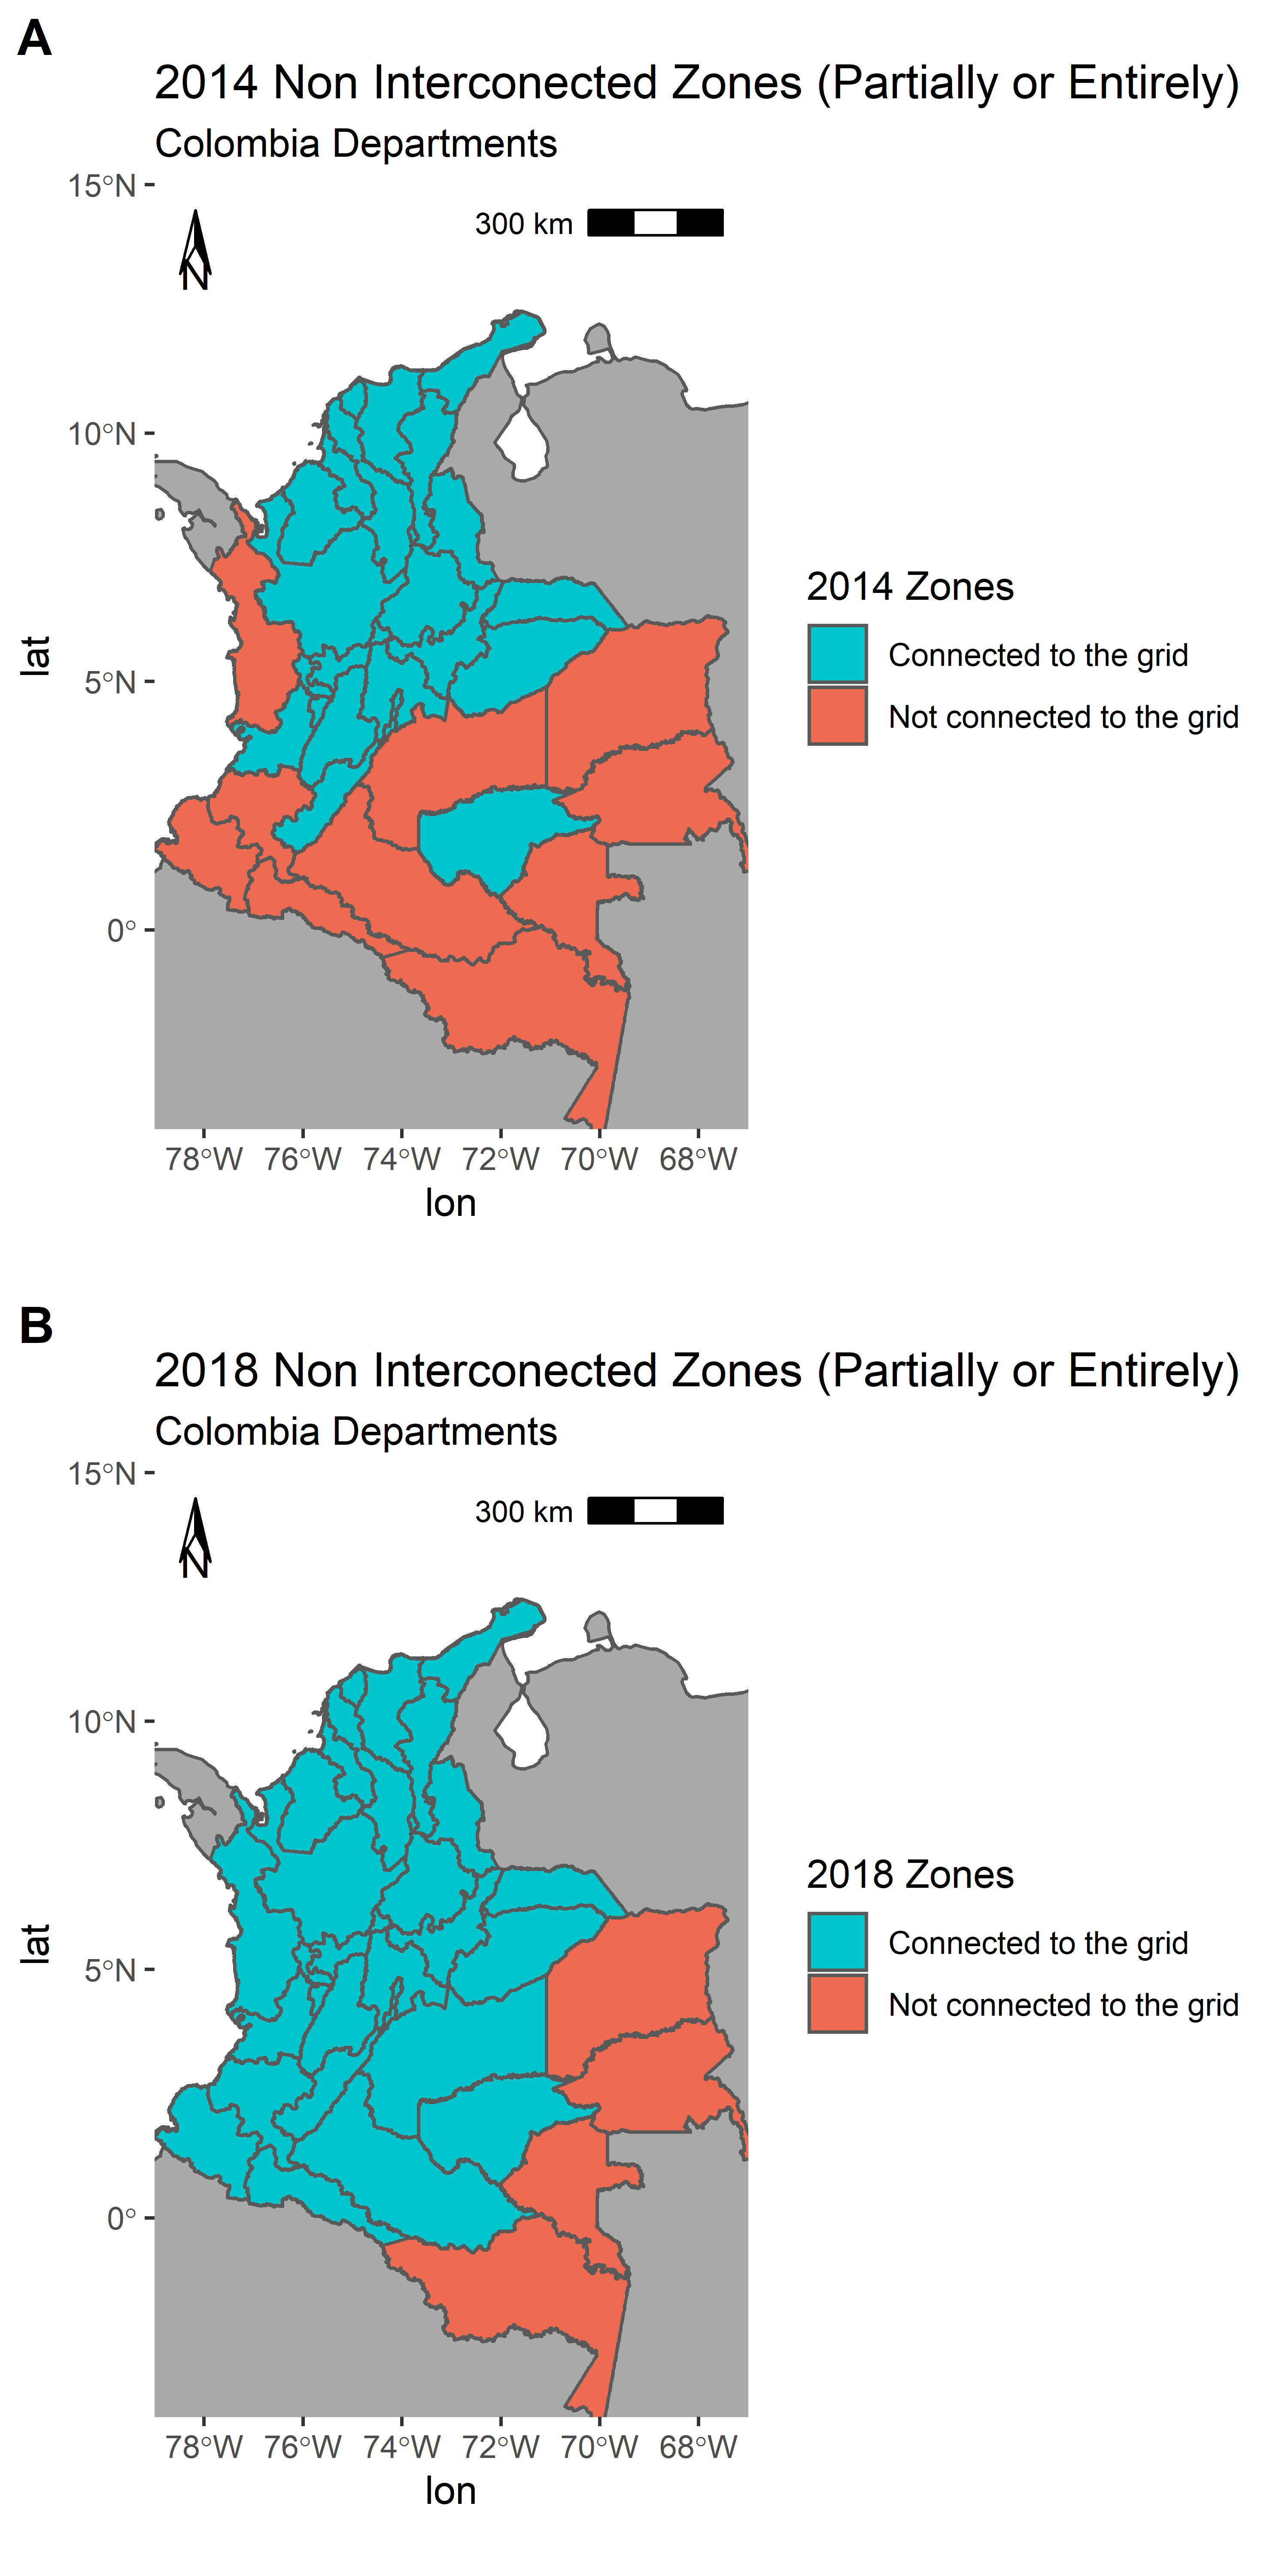
\includegraphics[width=8cm]{figs/non_interconnected_zones_v2.png}
	\caption{Energy access in Colombia. Zones partially or entirely non-connected to the national energy grid. A: 2014. B:2018. %MDPI: This figure is not mentioned in the main text. Please cite the figure in the text and ensure the first citation of each figure appears in numerical order. Please also add explanation for the subfigures. %Lina: Mentioned in the introduction.
	\label{fig:1}}
    \end{figure}
    


%\newpage


%%%%%%%%%%%%%%%%%%%%%%%%%%%%%%%%%%%%%%%%%%
\section{Materials and~Methods}

%Lina's changes: 'As previously mentioned' removed
%Lina's changes: Future tense verbs removed changed to present tense 
%Lina's changes: Removed 'as~previously mentioned in the literature review' 
%Lina's changes: Removed 'Previously, we have defined'

This article explores the use of second Generation GAMs to model spatial-temporal energy data with one-dimensional smoothers: Cubic Splines Cyclic and Non-Cyclic, and two-dimensional smoothers: Markov Random Fields and Tensor Splines, for the interactions used as case study data from Colombia. 
Smoothing splines through GAMs are more flexible than classically used GLMs, recognizing and characterizing non-linear relationships that can accommodate both space and time covariates~\citep{Amato2020ForecastingComponents}. Gaussian Markov Random Fields as Penalized Regression Spline make use of the penalty precision matrix to fit the smoothers to the~data.  \clearpage

     \subsection{One Dimensional Smoothers: Cubic Regression Splines Non-Cyclic and~Cyclic}
     A commonly used method for modelling time in energy demand modelling is the Cubic Regression Spline due to its high interpretability~\citep{Wood2017GeneralizedR}. Cubic splines are widely used in the literature to model non-linear relationships not only in the energy field but also in other fields as well~\citep{SalemJornaz2016ModelingComponents,Perperoglou2019AR}. Splines of degree df are defined as a continuous piecewise polynomial  \(b_1(x),b_2(x),…,b_k(x)\)  of the same degree with k basis functions, also called knots at \(\epsilon_1,…,\epsilon_k\) regions of the explanatory variable $x$ ~\citep{Hastie1999GeneralizedModels}.
     
     According to~Ref. \citep{Wood2017GeneralizedR} a spline can be represented as
\begin{equation}\label{eq:1}
     f(x)=\sum_{j=1}^{k}b_{j}(x)\gamma_{j}
     \end{equation}
where $b_j$  are the basis functions and $\gamma_j$ is the vector containing all the basis coefficients.~\citep{Perperoglou2019AR} reframes Equation~(\ref{eq:1}) based on not just the knots $k$ but also the degree of the spline $df$ as
\begin{equation}
    f(x)=\sum_{k=1}^{K+df+1}b_{k}(x)\gamma_{k}
     \end{equation}
     
     The idea of this is that with k knots there are $k+1$ polynomials of degree $df$, which makes the model have $k*df$ constraints, which generates $(k+1)(df+1)-k*df=k+df+1$ free parameters as pointed out by~Ref. \citep{Perperoglou2019AR}. In~a cubic spline  the degrees of freedom are therefore $k+4$.
     
     The representation of a cyclic spline is the same as for a cubic one, with the exception being that the limits of the summation do not go until the $k$, but until $k-1$ due to the cyclic end~condition
\begin{equation}
   f(x)=\sum_{j=1}^{k-1}\tilde{b_{j}}(x)\gamma_{j}
    \end{equation}
    
    Both cubic and cyclic spline have a second derivative that follows
\begin{equation} \label{eq:4}
   J(x)=\int_{x_1}^{x_k}f''(x)^2dx
	\end{equation}
	
 Equation~(\ref{eq:4}) is equivalent to \(\gamma^{T} D^{T} B^{-1} D\gamma\) if the spline is cubic and \(\gamma^{T}\tilde{D}^{T}\tilde{B}^{-1}\tilde{D}\gamma\) if the spline is cyclic cubic and they both can be summarized into \(\gamma^TS\gamma\) and \(\gamma^T \tilde{S}\gamma \), where $S$ and $\tilde{S}$ are the penalty matrices for each cubic and cyclic cubic spline,~respectively. 

  %  \newpage

     \subsection{Two Dimensional Smoother: Tensor Product Smooth~Interactions}
     All the concepts referred to in this section are derived from Ref. ~\citep{Wood2017GeneralizedR}.
     
     In order to include the interaction between the one-dimensional smoother, a tensor product smooth interaction was included.  If~there are two covariates $x$ and $z$ with smooth functions $f(x)$ and $f(z)$ with basis $b_{j}(x)$  and $a_m(z)$ such as
\begin{equation}
    f(x)=\sum_{j=1}^{k}b_{j}(x)\gamma_{j} \: and \: f(z)=\sum_{m=1}^{l} a_{m}(z)\delta_{m}  
    \end{equation}
    
    Therefore, the~smooth function of $f(x,z)$ can be represented as
\begin{equation}
    f(x,z)=\sum_{j=1}^{k}\sum_{m=1}^{l}b_{j}(x)a_{m}(z)\delta_{jm}
    \end{equation}
    
    This assumes that the vector containing the basis coefficients for $x$  $\gamma_{j}$ varies smoothly with $z$ such as
\begin{equation}
    \gamma_{j}(z)=\sum_{m=1}^{l}a_{m}(z) \delta_{jm}  
	\end{equation}
	
	The tensor product penalties are also derived from the associated penalty function for each covariate

\begin{equation}\label{eq:8}
	J(x)=\gamma^{T}S_{x}\gamma \; and \; J(z)=\delta^{T}S_{z}\delta
	\end{equation}
	leading to a double penalty based on the tensor product of Equation~(\ref{eq:8}) such as
\begin{equation}
	J_{x}(f(x,z))=\gamma^{T}\bar{S_{x}}\gamma \: and \: J_{z}(f(x,z))=\gamma^{T}\bar{S_{z}}\gamma
	\end{equation}
where $\gamma$ is the vector of $\gamma_{jl}$ arranged in the corresponding order according to covariates $x$ and $z$, $\bar{S_{x}}$ is the marginal penalty matrix for $x$ and $\bar{S_{z}}$ is the marginal penalty matrix for $z$. 

     \subsection{Two Dimensional Smoother: Markov Random~Fields}
     In a space where two-dimensional smoothers have to be used, Markov random fields can be fitted through a neighbourhood structure that works well with discrete geographic regions. 
     As stated by Ref.~\citep{Christakos2005RandomSciences} a random field, also called a stochastic field, is a collection of random variables \(X(s)={X(s_1),X(s_2),…,X(s_n)}\) at locations \(s_1,s_2,…,s_n\) \(s\in R^{n}\) where each random variable is defined on a probability space \((\Omega,F,P)\) where $\Omega$ is an abstract sample space also known as topological space, $F$ is a field of subsets of the abstract sample space $\Omega$ and $P$  is the probability measure on the space $(\Omega,F)$ that satisfies the Kolmogorov axioms: a)\(P(\Omega)=1\) , b) \(0<P(A_{i})<1\) for all sets \(A_{i} \in F\) and c) If \(A_{i} \in F\) and \(A_{i} \cap A_{j}=\varnothing\) then \(P(\bigcup_{i=1}^{\infty}A_{i} =\sum_{i=1}^{\infty}P(A_{i})\).
     
     The random fields range from Gaussian to Non-Gaussian and from Discrete to Continuous~\citep{Christakos2005RandomSciences}  and can be applied over space or time~\citep{Ibe2013MarkovEdition}. For~this application over discrete space lattice or areal regionally aggregated data, Gaussian random fields were preferred for being more intuitive when compared with non-Gaussian ones~\citep{Haran2011GaussianData}. 
     A Gaussian Random Field (GMRF), as defined by Ref.~\citep{Rue2005GaussianApplications}, is a random vector of $n$ finite dimensions \(X(s)={X(s_1),X(s_2),…,X(s_n)}\) for a finite set of locations \(s_1,s_2,…,s_n\) \(s \in R^{n}\)  that follows a multivariate Gaussian/Normal distribution \(X~N(\mu,\Sigma)\) with mean vector $\mu$ and positive definite covariance matrix $\Sigma$ such as
\begin{equation}
	\mu=E[X(s)]=
	\begin{pmatrix}
    E(X(s_1))\\
    E(X(s_2))\\
    ...\\
    E(X(s_n))
    \end{pmatrix}
	\end{equation}
	
	\begin{equation*}
	   \Sigma=Cov(X(s_i),X(s_j))
	\end{equation*}
\begin{equation}
	\begin{small}
	\begin{pmatrix}
	Cov(X(s_1),X(s_1)) & Cov(X(s_1),X(s_2)) &  ... & Cov(X(s_1),X(s_n))\\
	Cov(X(s_2),X(s_1)) & Cov(X(s_2),X(s_2)) &  ... & Cov(X(s_2),X(s_n))\\
	... & ... & ... & ... \\
	Cov(X(s_n),X(s_1)) & Cov(X(s_n),X(s_2)) &  ... & Cov(X(s_1),X(s_n))
	\end{pmatrix}
	\end{small}
	\end{equation}
	
	The multivariate normal distribution for the random vector $X(s)$ of n finite dimensions with the mean vector $\mu$ and covariance matrix $\Sigma$ is the following
\begin{equation}
    p(X)=\frac{\Sigma^{-1/2}}{2\pi^{n/2}}exp\Big\{-\frac{1}{2}(X-\mu)^{T} \Sigma^{-1} (X-\mu)\Big\}
    \end{equation}
    
    The Gaussian Random Field (GMRF) can also be defined in terms of a sparse matrix allowing the employment of sparse matrix solution techniques and properties and ultimately a faster computation, as indicated by Ref.~\citep{Rue2005GaussianApplications}. The~precision sparse matrix, in~this case would be the inverse of the covariance matrix such as $Q=\Sigma^{-1}$, making the model become $X~N(\mu,Q^{-1})$. The~multivariate Normal distribution for the random vector $X(s)$ of n finite dimensions when using the precision sparse matrix $Q$ instead of the covariance matrix $\Sigma$  could be expressed~as
    
    \begin{linenomath}
\begin{equation} \label{eq:13}
    p(x)=\frac{ |Q |^{1/2}}{2\pi^{n/2}} exp\{-\frac{1}{2}(X-\mu)^{T}Q(X-\mu)\}
    \end{equation}
    \end{linenomath}
    
    This finite set of locations \(s_1,s_2,..,s_n\) \(S \in R^{n}\) from the Gaussian Random Field (GMRF) are defined within a neighbourhood structure that is represented through an undirected labelled graph \(g=(v,\epsilon)\) where $v$ is a set of labelled nodes/regions \(v={1,...,n}\) and $\epsilon$ is a set of undirected edges from node $i$ to node $j$ ${i,j}$ where \(i,j \in v\) and $i \neq j$ n the case of areal data the edges are the spatial borders between the~regions.
    
    If the regions share a common border, then the sparse matrix is non-zero $Q_{ij} \neq 0$ and the regions $i$ and $j$ are neighbours such as \(ne(i)=j \Longleftrightarrow ne(j)=i\), which can also be expressed as  \(i \sim j \Longleftrightarrow j \sim i\). It can be said that the neighbouring regions $i$ and $j$ are conditionally dependent such as \(p(x_i \vert x_j)\) when \(i,j \in v \: and \: i \neq j\).
    
    If regions $i$ and $j$ do not share any spatial border, then there is no edge between $i$ and $j$, and then the sparse matrix is zero \(Q_{ij}=0\), and that \(x_i \bot x_j \vert x_{-ij}\) for all \(i \neq j\), which means that the regions $i$ and $j$ are not neighbours and are conditionally independent of all the other regions in the neighbourhood structure, and \(x_{-ij}\) indicates all elements except for $i$ and $j$. %please verify
    
    For the case presented here, a fully connected neighbourhood structure is assumed, which can be represented through a fully connected undirected labelled graph, in which \({i,j} \in \epsilon\) for all \(i,j \in v\) with \(i \neq j\). %please verify


    
    Figure \ref{fig:2} %MDPI: Please check if the figure's label is missing %Lina: Added reference to figure 2
    represents an areal data neighbourhood structure with 14 nodes or regions such as \(v=\{0,1,2,3,4,5,6,7,8,10,11,12,13,14\}\) and with 29 as the set of edges or boundaries between~regions
    
    \begin{equation*}
    \epsilon =
    \begin{Bmatrix}
        \{7,13\}, & \{7,2\}, & \{13,2\}, & \{13,11\}, \\
        \{13,3\}, & \{13,6\}, & \{2,12\}, & \{2,11\} \\
        \{12,11\}, & \{12,8\}, & \{11,8\}, & \{11,0\} \\
        \{11,3\}, & \{8,0\}, & \{8,1\}, &  \{6,14\}\\
        \{10,14\}, & \{10,4\}, & \{14,4\}, & \{4,5\} \\
        \{5,1\}
    \end{Bmatrix}
    \end{equation*}
    

    As can be seen in Figure~\ref{fig:2}, region 7 is a neighbour of regions 2 and 13 such as \(nei(7)=\{2,13\}\), region 13 has as neighbours the regions 7, 2, 11, 3, and~6 such as \(nei(13)=\{7,2,11,3,6\}\), and so on. The~average amount of neighbours for this neighbourhood structure is four, with a minimum of two neighbours in region 7 and a maximum of seven neighbours in region 0, such as \(nei(0)=\{11,8,3,14,4,5,1\}\).
    \vspace{-12 pt} 


    \begin{figure}[H]
	%\centering
\hspace{-2em}
    \centering
		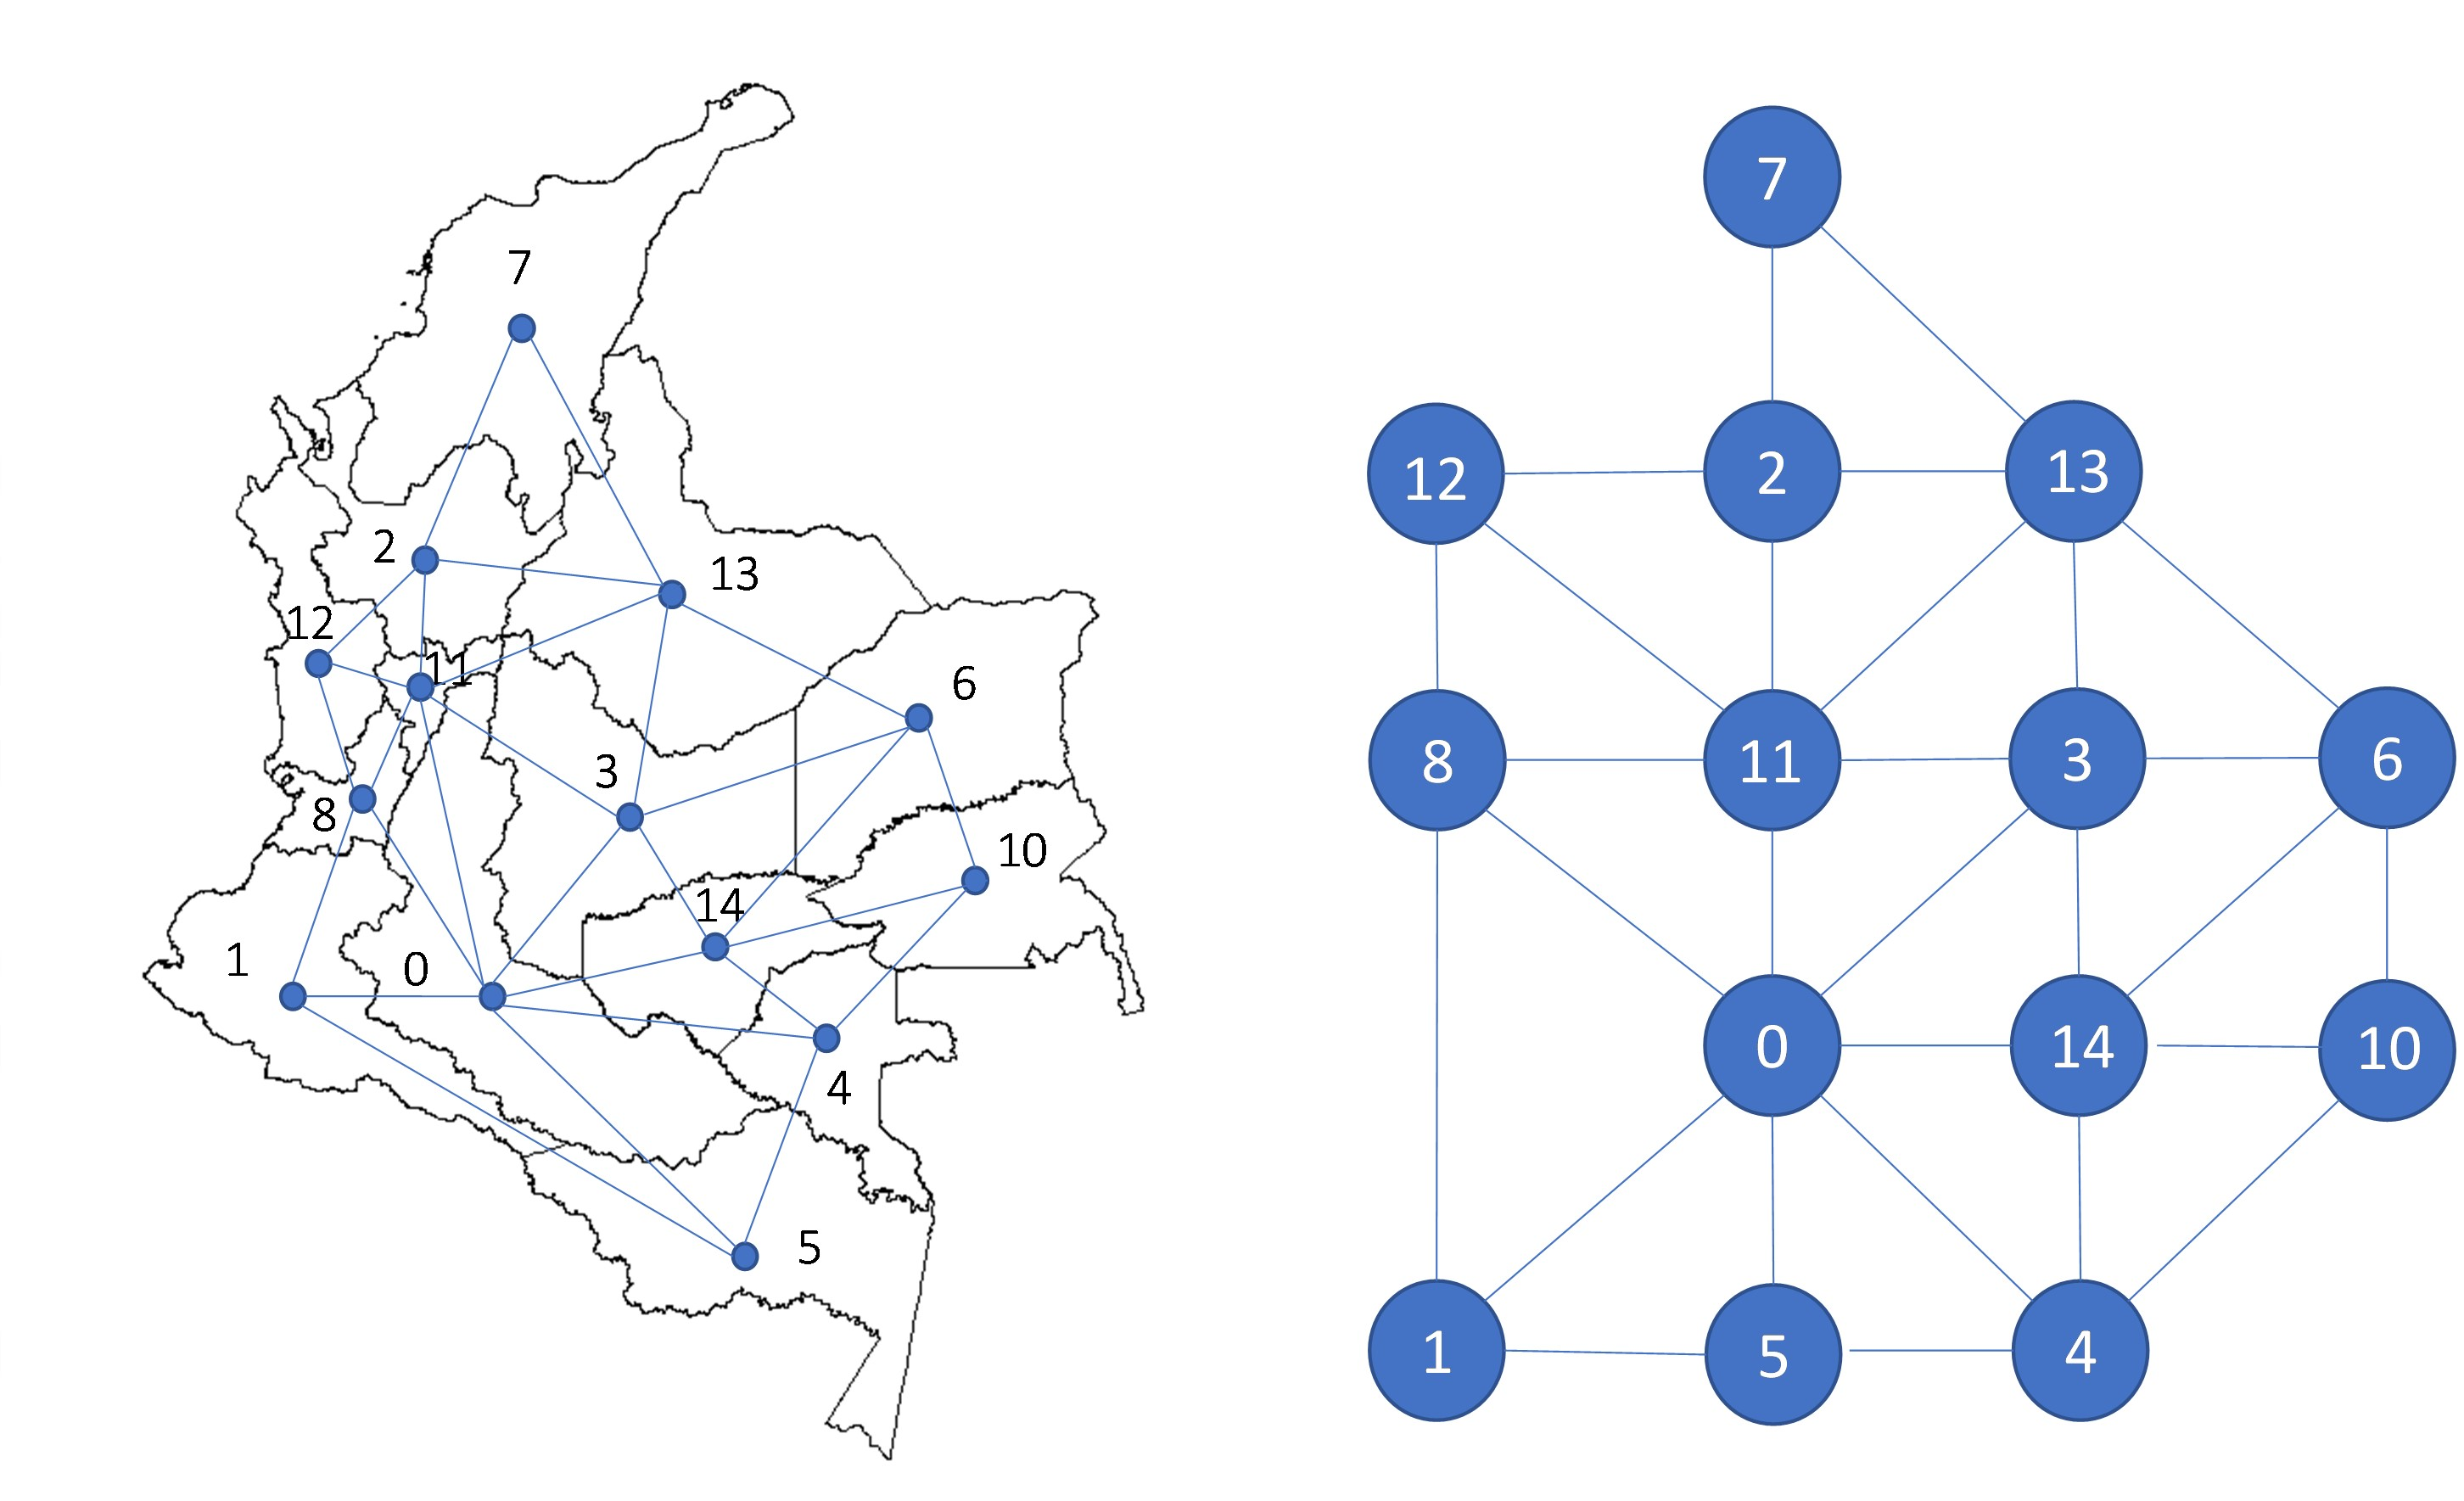
\includegraphics[scale=.85]{figs/Markov_Random_Fields.jpg}
	\caption{Neighbourhood structure relationship applied to Colombia. Regions form an irregular lattice. The~left column shows the conditional dependence between the connected regions while the right column translates it to~nodes. \label{fig:2}}
    \end{figure}

%%%%%%%%%%%%%%%%%%%%%%%%%%%%%%%%%%%%%%%%%%
\section{Results}

The demand data in this study is kilowatts hourly information collected monthly and published yearly by the entity that oversees the grid of the electricity sector in Colombia~\citep{XMHistoricalDemand}(See figure \ref{fig:3}).

    \begin{figure}[H]
	%\centering
%\hspace{-1em}
		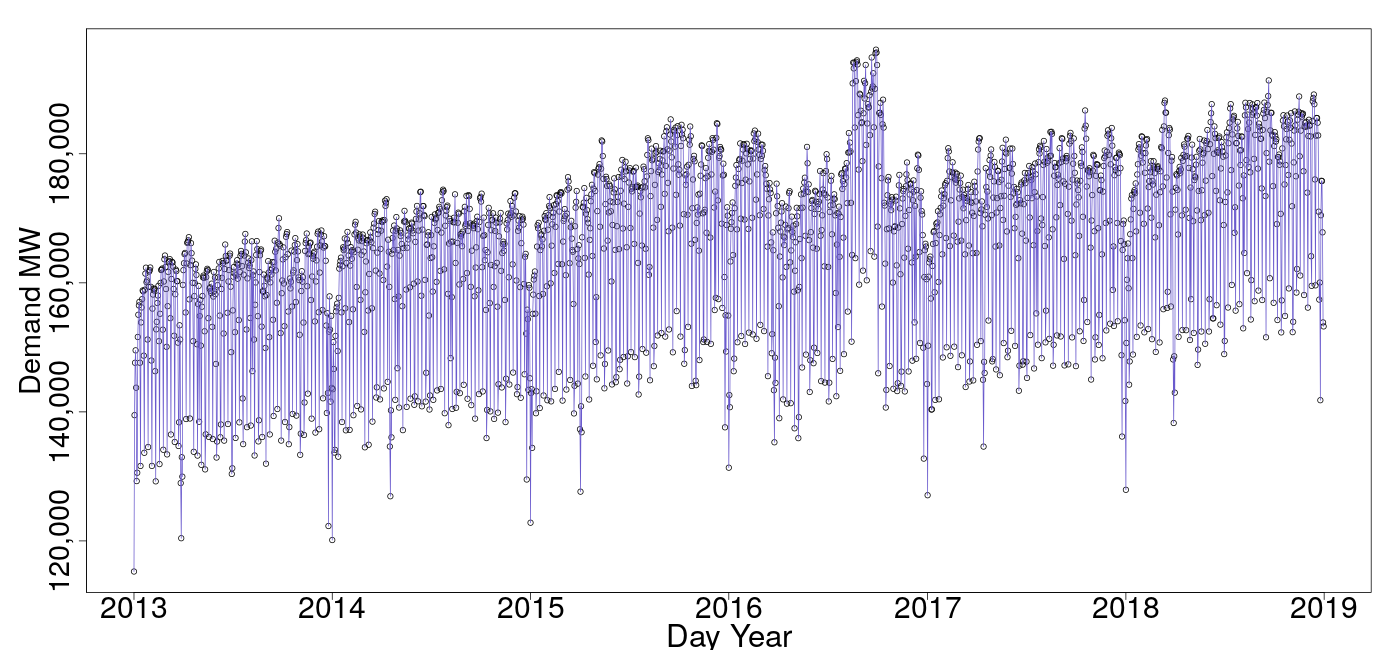
\includegraphics[height=6cm, width=14cm]{figs/timeseriesdemand.png}
	\caption{\hl{Unsmoothed} %MDPI: Please use commas to separate thousands for numbers with five or more digits (not for four digits) in the picture. e.g., "10000" should be "10,000"
 \hl{data} %MDPI: This figure is not mentioned in the main text. Please cite the figure in the text and ensure the first citation of each figure appears in numerical order. %Lina: Figure cited and moved to the beginning of results section
 from January 2013 to December~2018. \label{fig:3}}
    \end{figure}

%Lina's changes: Changed numbers to words acording to APA
The input data used for both spatial and temporal regressions are hourly aggregated information for each department by day in a range of five years from 2013 to 2018 . No disaggregated information from smaller administrative areal units such as municipalities or point data about home consumption was available. The thirty-two departments were grouped into fifteen regions for this analysis, as shown in Table~\ref{tab15} from Appendix.

     \subsection{Non-Spatial GAM: Generalized Additive Model Regression Using Cubic Splines as a One-Dimensional Smoother for Modelling~Time} 
     
     Additive models were introduced by Ref.~\citep{Stone1986TheModels} to deal with the dimensionality problem of the General Linear Models GLMs through univariate smoothing~\citep{Nisbet2018BasicOverview}. The~GAMs Stone approach can be seen as a  traditional way of portraying GAMs, which in this case has the demand as the response variable d, and space or time as predictors $x_j$, which can be written as
\begin{equation}
        d=\alpha_{0}+f_1(x_1)+f_2(x_2)+...+f_k(x_k)+\epsilon
     \end{equation}
or its summarised version
\begin{equation}
         d=\alpha_{0}+\sum_{j=1}^{k}f_j(x_j)+\epsilon
     \end{equation}
where \(\alpha_{0}=E[f(x)]\) and $f_j$ are the smooth functions over the covariates $x_j$.
     
     The Stone approach fails to include interaction and therefore has unsatisfactory results when interaction exists~\citep{Faraway2006ExtendingModels}. It is here that the approach from~Ref. \citep{Hastie1999GeneralizedModels} becomes important, as it not only includes interactions $f_j$ but also includes the  link function g over the response variable $d$ to analyse $x_j$  within a solution space of any member of the exponential family, usually Gaussian-Normal, but it is open to Gamma, Poisson, or~Binomial~\citep{Nisbet2018BasicOverview}. Then, a Generalized Additive model over the demand according to the Hastie and Tibshirani approach can be written as
\begin{equation}
     g(\mu)=\alpha + \sum_{j=1}^{k}f_j(x_j)+ \epsilon
     \end{equation}
where  $f_j$ are the smooth functions over the covariates $x_j$ allowing for both single basis smoothing \(\sum_j f_j (x_j)\) and interactions \(\sum_{j \neq i}f_j (x_i,x_j)\) and \(\mu=E(d)\). In~this approach, $\alpha$ is a regression for the variables that will not be modelled additively. %please verify
  Hastie and Tibshirani defineed the procedure for estimating $\alpha$ and $f_j$ as a local scoring procedure for generalized additive~models.
     
     In the early 2000s, Ref.~\citep{Wood2006GeneralizedR} provided a more recent perspective to the GAM definition developed by Ref.~\citep{Hastie1999GeneralizedModels}, denoted in Equation~(\ref{eq:13}). The author %please verify
      directly defined the iterative procedure with a model structure that has index $i$, in which $\alpha$ is represented as the product of the model matrix $A$ and a vector of the associated model parameters $\theta$, where the intercept is assumed to be included. $A$  is a design matrix for the covariates $x$ with linear effects. The author also included a linear operator $L_ij$ to multiply the smooth function $f_j$. %please verify
\begin{equation}\label{eq:17}
         g(\mu_i)=A_i\theta+ \sum_{j=1}^{k}L_{ij}f_{j}(x_{j})+\epsilon_{i}
     \end{equation}
where $d_i$ is distributed according to an exponential family EF that has median $\mu_i$   and variance $\phi$ ,  \(d_i \sim EF(\mu_i,\phi)\).
     
     The cubic regression spline smoother is represented through the function $f_j$ where $b_j$ is a base function of the spline and $\gamma_j$ is the vector containing all the basis coefficients such as
\begin{equation}
         f_j(x_j)=\sum_{j=1}^{k}b_j(x)\gamma_j
     \end{equation}
     
     Finally, a vector of coefficients  $\gamma$ that contains the linear fixed effects vector $\theta$ followed by all the basis coefficients $\gamma$ for $f_j$  such as \(\gamma=\{\theta,\gamma_1,...,\gamma_k\}\) is defined. Then the estimation of the vector of coefficients $\hat{\gamma}$ from the GAM model will be done by penalized maximum likelihood, where the optimal is given by some smoothing parameters $\delta_j$~\citep{Wood2006GeneralizedR}
\begin{equation}
         \hat{\gamma}=argmin_{\gamma} \Bigg( D(\gamma)+\sum_{j=1}^{k}\delta_j\gamma^TS_j\gamma \Bigg )
     \end{equation}
where $S_j$ is a penalty matrix and the deviance of the model \(D(\gamma)=2(l(\gamma_max )-l(\gamma))\phi\)
     
     Note that not only the optimal vector of coefficients $\hat{\gamma}$ must be estimated but also the parameters themselves  $\delta_j$. The~smoothing parameters estimation $\delta_j$ is done either by prediction error criteria (GCV) or maximum likelihood (ML or REML)~\citep{WoodGamDocumentation}.
     
     The method that we will be used in this article for selecting the smoothing parameters  $\gamma_j$  is the Restricted Maximum Likelihood, REML. This will be done instead of other smoothness selection methods such as ML, Maximum Likelihood, and GCV, Generalized Cross-validation.  %please verify
       In~REML unlike ML, the estimation of variance components is better, as it has a higher probability of providing a complete rank of estimates of the variance components~\citep{Vasdekis2005OnData}. On~the other hand, REML is preferred over GCV  due to it having a higher penalty for overfitting and being less likely to have multiple minimum points, therefore being less likely to have highly variable smoothing parameters $\lambda_j$ ~\citep{Wood2010FastGLMs}.
    
    In the literature, demand electricity is usually modelled by three patterns: daily, weekly, and~monthly. Ref. ~\citep{Meier2019Short-termModels} modelled the previously mentioned patterns through a GAM by preselecting the knots according to the number of unique values of the variables included in the model. In that case, when~modelling the patterns, only continuous variables were included with 24~knots for the daily pattern, 7~knots for the weekly pattern, and~12~knots for the monthly pattern. In this case, the~daily pattern was included in the model through an hour variable, the~weekly pattern through a categorical variable that differentiates days between weekend and weekdays, and instead of including a monthly pattern a trend pattern was included. In~the model, the interactions between categorical and numerical variables were included. Knots were not set up based on unique values but on sensible values according to the underlying~data.
    
    Initially, the~daily pattern was included in the model using a cyclic spline smooth over the discrete variable hour with a range from 0 to 23, $s(hr,bs=cc,k=24)$. After~this, the~weekly pattern was included in the model as a categorical variable, wk, where weekly days were classified as 1-Monday and 7-Sunday, and were aggregated into two factors, $wk/wknd$. The~corresponding interaction between the discrete numerical variable that accounts for the daily pattern, hr, and the categorical variable, wk, that accounts for the weekly pattern was also included using a factor smooth-interaction with the argument inside the smooth function, s, in the following way $s(hr,bs=cc,by=wk,k=24)$. Finally, trend pattern was fitted not by using the month's numeric notation from 1 to 12 or the days of the year from 1 to 365, but through a trend variable that goes from 1 to 43,800, that accounts for the total number of data points available days per years per hour between 2013 and 2018 %please verify Lina: Changed
    through a cubic spline smooth $s(time,bs=cr,k=10)$. The~interaction between the daily pattern and the trend pattern was fitted using pairwise bivariate tensors product interactions $ti(hr,time,bs=c(cc,cr),k=c(24,10))$. 
    
    This model can be expressed as
\begin{equation}
    \begin{split}
        g(\mu_i)=A_i+f_1^s(hour)+weekday+f_3^T(time)\\+f_{1,2}^I(hour by weekday)+f_{1,3}^I(hour,time)
    \end{split}
    \end{equation}
where $A_i\theta$ accounts for the linear effects and the f function accounts for the non-linear effects defined by each smoothed covariate. The~super indexes $S,T and I$  correspond respectively to the Seasonal, Trend, and~Interaction components. In~the model \(\mu_i=E(d_i )\) with the response variable demand being distributed as \(d_i~N(\mu_i,\phi)\).
    
    As can be seen in \hl{Table}%MDPI: Tables 1 and 2 have to be mentioned before Table 3. Please revise. %LIna: It was referring to table 1
    ~\ref{tab1}, the~resultant temporal model accounts for eighty-five percent of the electricity demand~variation.

    \begin{table}[H] 
    \caption{Model summary table for non-spatial~GAM. \label{tab1}}
    \newcolumntype{C}{>{\centering\arraybackslash}X}
    \begin{tabularx}{\textwidth}{CCCCC}
    \toprule
    \textbf{Rsq} & \textbf{Dev} & \textbf{\hl{REML} %MDPI: Please use scientific notations (e.g., "$8 \times 10^{3}$", not "8E3"). 
} & \textbf{Scale Est} & \textbf{n}\\
    \midrule
    0.852 & 0.853 & $7.573 \times 10^{5}$ & $1.874 \times 10^{11}$ & 52,584\\
    \bottomrule
    \end{tabularx}
    \end{table}
    
    The Wald \emph{t}-test in Tables~\ref{tab2} and \ref{tab3} for the non-spatial GAM model shows that all smooth terms and parametric terms are highly~significant.

    \begin{table}[H] 
    \caption{Parametric coefficients for non-spatial~GAM.\label{tab2}}
    \newcolumntype{C}{>{\centering\arraybackslash}X}
    \begin{tabularx}{\textwidth}{cCCCC}
    \toprule
    \textbf{Var} & \textbf{Estimate} & \textbf{Std.Error} & \textbf{\emph{t}-Value} & \textbf{\hl{Pr} %MDPI: Please use scientific notations (e.g., "$8 \times 10^{3}$", not "8E3"). 
}\\
    \midrule
    Intercept & 7,146,219
 & 10,848 & 658.8 & $<2 \times 10^{-16}$\\
    weekday (wk/wknd) & $-$697,836 & 4180 & $-$166.9 & $<2 \times 10^{-16}$\\
    \bottomrule
    \end{tabularx}
    \end{table}
\unskip
    
    \begin{table}[H] 
    \caption{Smooth terms/non-parametric coefficients for non-spatial~GAM.\label{tab3}}
    \newcolumntype{C}{>{\centering\arraybackslash}X}
    \begin{tabularx}{\textwidth}{cCCCC}
    \toprule
    \textbf{Var} & \textbf{Estimate} & \textbf{Std. Error} & \textbf{\emph{t}-Value} & \textbf{\hl{Pr} %MDPI: Please use scientific notations (e.g., "$8 \times 10^{3}$", not "8E3"). 
}\\
    \midrule
    hour-s(hr) & 21.2287 & 22.000 & 56.312 & $<2 \times 10^{-16}$\\
    hour by weekday-s(hr):wk/wk & 18.5862 & 22.000 & 12.482 & $<2 \times 10^{-16}$\\
    hour by weekday-s(hr):wk/wknd & 0.6319 & 22.000 & 0.029 & $7.63 \times 10^{-15}$\\
    time-s(time) & 8.8768 & 8.981 & 142.593 & $<2 \times 10^{-16}$\\
    inter hour and time-ti(hr,time) & 90.1125 & 198.000 & 4.785 & $<2 \times 10^{-16}$\\
    \bottomrule
    \end{tabularx}
    \end{table}
\unskip
    
    The knots were preselected, but not based on unique values, as in Ref.  ~\citep{Meier2019Short-termModels}, but on sensible values that reduce the heteroscedasticity of the data as much as possible while maintaining them at logical levels below 24~knots. Splines over 10~knots are rare and can lead to model overfitting, so in~this case the~upper limit was set  to 24 because of the number of unique values of the variable hours. Previous literature also points out that selecting unique values for time related variables makes a better~fit. 
     
    Heteroscedasticity which indicates if the basis dimension \emph{k} is too low, was checked through the $k$-index in Table~\ref{tab4}. The model was divided between the residual variance to get a $p$-value. 

    \begin{table}[H] 
    \caption{K-check for non-spatial~GAM. \label{tab4}}
    \newcolumntype{C}{>{\centering\arraybackslash}X}
    \begin{tabularx}{\textwidth}{cCCCC}
    \toprule
    \textbf{Var} & \textbf{\emph{k}} & \textbf{edf} & \textbf{\emph{k}-Index} & \textbf{\emph{p}-Value}\\
    \midrule
    s(hr) & 22 & 21.2287 & 0.9827 & 0.1175\\
    s(hr):wk/wk & 22 & 18.5861 & 0.9827 & 0.1075\\
    s(hr):wk/wknd & 22 & 0.6318 & 0.9827 & 0.1050\\
    s(time) & 9 & 8.8768 & 0.8344 & 0.0000\\
    ti(hr,time) & 198 & 90.1124 & 0.8369 & 0.0000\\
    \bottomrule
    \end{tabularx}
    \end{table}

    The hours variable and its respective interactions showed no evidence of heteroscedasticity with a $p$-value over zero. On~the other hand, the~number of data points was clearly heteroscedastic with a \emph{p}-value around zero. For~reducing heteroscedasticity in the model, it was attempted to increase the number of knots for the data points variable up to 50, but~this had little to no effect in the \emph{k}-index or \emph{p}-value. Fifty knots were chosen as an upper limit to test the heteroscedasticity values due to it accounts of two years of data. Going above this value was not explored because the size of the data does not call for a high number of knots, considering that there were only five years~available. The residual vs. fitted plot (See Figure \ref{fig:4} - second plot from left to right) also shows proofs of heteroscedasticity or non-constant spread in the~data.  

    
    \begin{figure}[H]
	%\centering
%\hspace{-1em}
		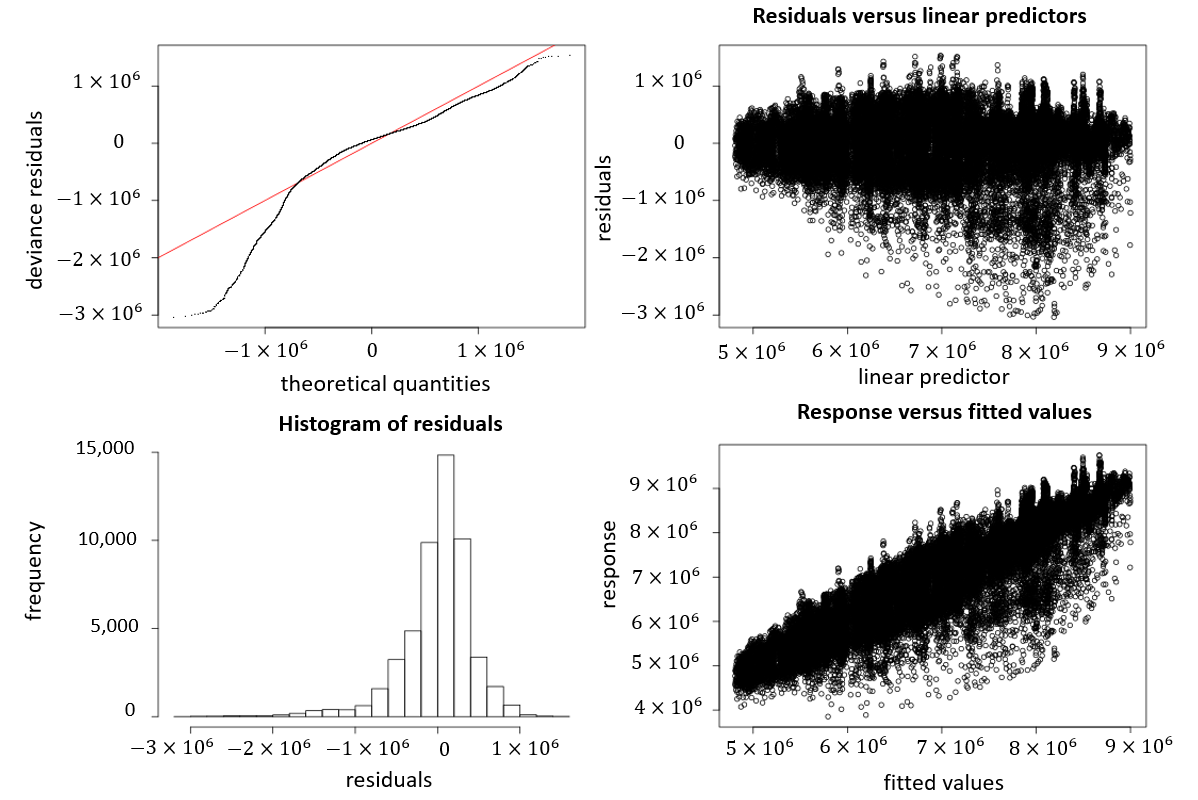
\includegraphics[height=6cm, width=14cm]{figs/diagnosticplot.png}
	\caption{\hl{Diagnostic} %MDPI: The contents of this figure are not legible. In order to convert a clear PDF document, whilst retaining its high quality, we kindly request the provision of figures and schemes at a sufficiently high resolution (min. 1000 pixels width/height, or a resolution of 300 dpi or higher).
 \hl{plot} %MDPI: This figure is not mentioned in the main text. Please cite the figure in the text and ensure the first citation of each figure appears in numerical order. %Lina: Cited
 for non-spatial~GAM. \label{fig:4}}
    \end{figure}
    
    The model demonstrated convergence after ten iterations supporting the data being enough for the number of parameters. However, by looking at the Autocorrelation Function (ACF) and Partial Autocorrelation Function (PACF) it can be seen there is remaining autocorrelation that the model is not capturing (See Figure~\ref{fig:5}).

    \begin{figure}[H]
	%\centering
%\hspace{-1em}
		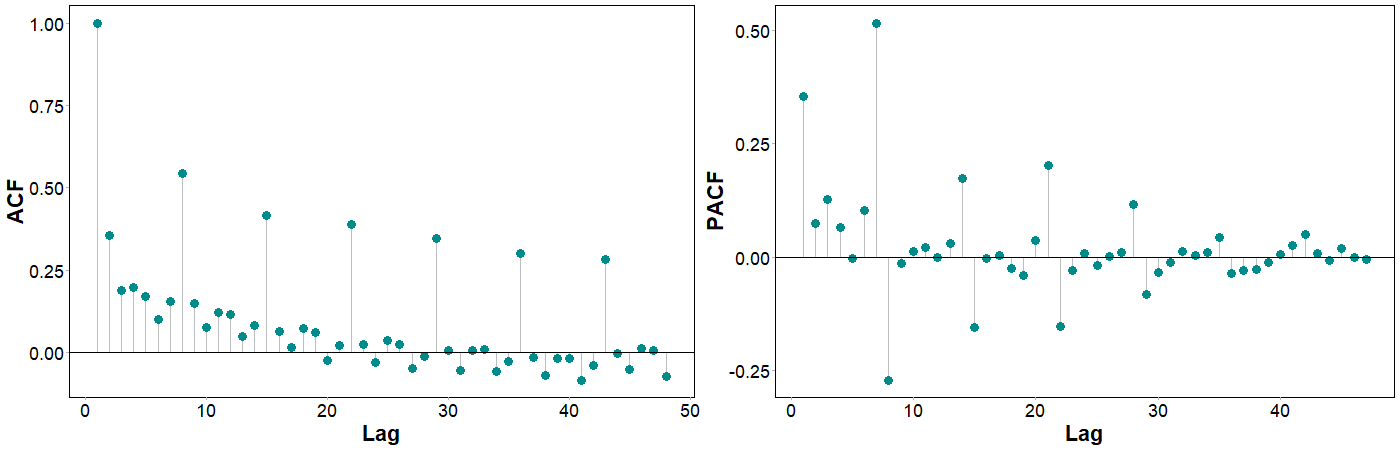
\includegraphics[height=4cm, width=14cm]{figs/Autocorrelation_Residuals.png}
	\caption{\hl{Autocorrelation} %MDPI: Please consider replacing this figure with a sharper version of it.
	\hl{residuals} %MDPI: Please change the hyphen (-) into minus sign ($-$, "U+2212") if possible. e.g., "-1" should be "$-$1". %Lina: That is how the ACF and PACF are always represented. This is the traditional way of showing autocorrelation.
 of non-spatial~GAM. \label{fig:5}}
    \end{figure}
        
    As is the case for GAMs, the correlation among covariates was tested through concurvity instead of collinearity due to the non-linear nature of the model. As~expected, there is acceptable concurvity between individual effects and interactions (See Figure ~\ref{fig:6}). There is no reason to believe that smooth terms of the model approximate to other~terms. 

    \begin{figure}[H]
	%\centering
%\hspace{-1em}
   \centering
		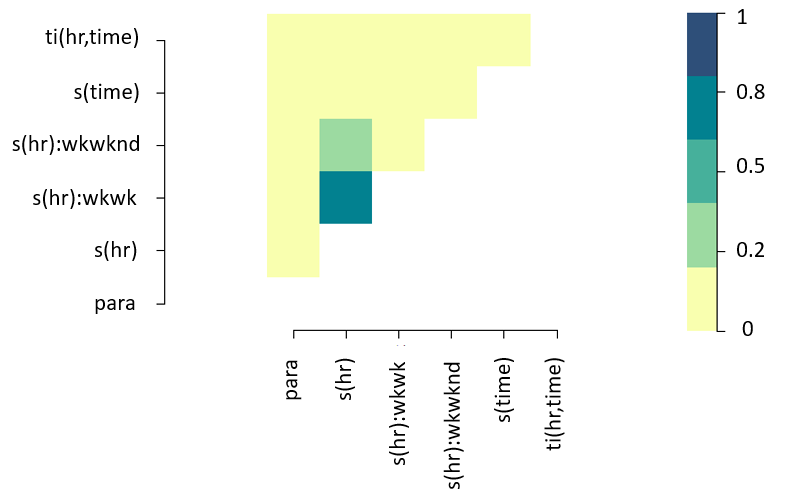
\includegraphics[height=7cm, width=10cm]{figs/Pairwise_Estimated_Concurvity.png}
	\caption{Pairwise estimated concurvity of non-spatial~GAM.\label{fig:6}}
    \end{figure} 

    \hl{Figure}%MDPI: FIgure 6 has to be mentioned before Figure 7. Please revise and move the figure below its first citation. %Lina: There were two figures with the same label. I just corrected it.
    ~\ref{fig:7} exhibits flat line in the density graph (first line, third figure) for the interaction of hours and weekend indicating there is no much of an effect in the interaction of such variables.On~the contrary, the~interaction between hours and weekdays shows a clear spline pattern in the density graph (first line, second figure). Both the individual effects of hours and data points portrayed in the first figures of the first line and second line show splines with a higher degree of curvature than the~interactions. 

     \begin{figure}[H]
	%\centering
		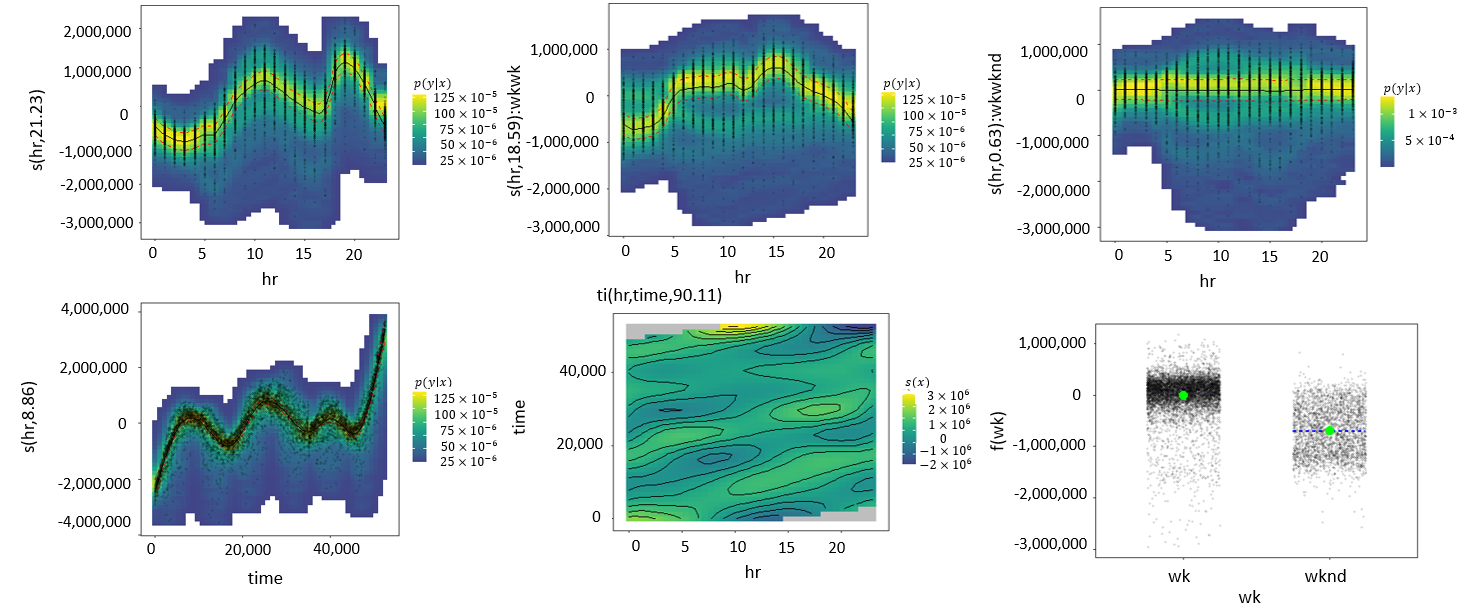
\includegraphics[height=9cm, width=14.5cm]{figs/Partial_Effects_Plot_Non_Spatial.png}
	\caption{\hl{Partial} %MDPI: Please consider replacing this figure with a sharper version of it.
         \hl{effects} %MDPI: Please change the terms into scientific notation in the figure if possible. (e.g., "$8 \times 10^{3}$", not "8E3"). %Lina: Notations were changed and quality was improved
        for the non-spatial GAM: effects for individual covariates, interaction covariates, and~parametric factor~term. \label{fig:7}}
    \end{figure}
\unskip
    
    
     \subsection{Spatial GAM: Generalized Additive Model Regression Using Markov Random Fields as a Two-Dimensional Smoother for Modelling~Space}

     %Lina's changes: in this dissertation --> in this article
     
     Often, space modelling is associated with Geographically Weighted Regression,  \linebreak GWR~\citep{Fotheringham2002GeographicallyRelationships}, which according to~Ref. \citep{Fahrmeir2004PENALIZEDPERSPECTIVE} is based on the Varying Coefficient Model, VCM proposed by~Ref. \citep{Hastie1993Varying-CoefficientModels}. Although~there are many other types of modelling such as the Geoadditive model~\citep{Kammann2003GeoadditiveModels}, this one is specifically based on GLMs. In~this article, the space modelling is going to be based on GAMs, as proposed by Refs. ~\citep{Fahrmeir2004PENALIZEDPERSPECTIVE,Fahrmeir2011BayesianData} and later incorporated by Ref.~\citep{Wood2017GeneralizedR}. 
     
     
     The spatial modelling will be performed through GAM using GMRF over areal data, which is often considered a separate spatial modelling technique~\citep{StockWhatRisk} but in this case it was incorporated to the Generalized Additive Model  as a two dimensional smoother so it can account for the model covariance as a function of the location, as proposed by Refs.  ~\citep{Fahrmeir2011BayesianData,Wood2017GeneralizedR}. 
     
     \textls[-15]{Areal data is important for its various applications not only in the energy demand fields where observations could be allocated to a region according to the electricity operator but also to census and survey data where observations are aggregated to administrative~districts.}
     
     Spatial GAM has the same structure as a non-spatial GAM with the addition of a term that accounts for the spatial effect represented through the smooth function $fspat(s_i)$~\citep{Fahrmeir2011BayesianData} such as
\begin{equation}\label{eq:20}
        g(\mu_i)=A_i\theta+\sum_{j=1}^{k}L_{ij}f_j(x_j)+fspat(s_i)+\epsilon_i
     \end{equation}
    where \(d_i \sim EF(\mu_i,\phi)\)
    
    In Equation~(\ref{eq:20}), $A_i\theta$ accounts for the linear effects of covariates $x$ while \(\sum_{j=1}^{k}L_{ij}f_j(x_j)\) accounts for the non-linear deterministic effects defined by the smoothers and $fspat(s_i)$ accounts for the spatially correlated effect that in the equation is calculated by the~GMRF. %please verify
    
    
    Here the dependence of all the terms from the spatial locations is suppressed for simplicity, but it is assumed when including the Gaussian stochastic process assumptions through $fspat(s_i)$, therefore no subindex $s$  related to the locations is~included.
    
    Equation~(\ref{eq:20}) can also be represented in terms of the vector of spatial effects $v$~\citep{Fahrmeir2011BayesianData} through an incidence matrix $R_{i}$, which ensures that each observation is assigned the spatial effect of the corresponding $s$ region it belongs to by assigning ones or zeros according to whether that observation $i$ has been collected in that region $s$ or not
\begin{equation}
        R_i=R[i,s]=
    \begin{cases}
    1 \\
    0
    \end{cases}
    \end{equation}
which translates to
\begin{equation}\label{eq:22}
        g(\mu_i)=A_i\theta+ \sum_{j=1}^{k}L_{ij}f_j(x_j)+R_iv+\epsilon_i
    \end{equation}
    
    After establishing the Generalized Additive Model, GAM, this article will proceed to explain the assumptions under the spatially varying effects vector, $v$.
    
    To understand how the spatially varying effects vector $v$ operates and its underlying assumptions, it is necessary to briefly recapitulate the fact that the spatial effect vector forms part of a spatial function $fspat(s_i)$ expressed as $R_iv$ for the specific case of discrete spatial areal data. 
    $v$ distribution follows a Gaussian Markov Random Field, GMR,F prior distribution conditional on the variance parameter $\tau^2$~\citep{Fahrmeir2004PENALIZEDPERSPECTIVE}. In \hl{numeral}~2.3,%MDPI: Please check if this is the citation of Section 3.3. %Lina: Change to 2.3
     it was mentioned how Gaussian Markov Random Fields, GMRFs, follow a multivariate normal distribution such as \(X~N(\mu,\Sigma)\). In~this case the multivariate normal model does not fully specify the join distribution of $\gamma$ because the variance $\Sigma$ is known and denoted as $\tau^2$,  but $\mu$ is a completely unknown reason, which is why we say that the prior is an improper prior, making the Gaussian Random Field be an Intrinsic Gaussian Random Field,  IGMRF~\citep{Faulkner2018LocallyPriors}. The~use of improper prior distributions is widely done and preferred in Bayesian statistical analysis when the information about parameters is weak or missing~\citep{Held2020LikelihoodInference}.
    According to Ref.~\citep{Rue2005GaussianApplications}, Intrinsic Gaussian Random Fields, IGMRFs, can be defined in both regular or irregular lattice. A~lattice is a structure or pattern for arranging an area of land into spatial units called sub-areas, cells, or~units~\citep{Saveliev2007AnalysisData}. As~stated in~Ref. \citep{Saveliev2007AnalysisData} these sub-areas share boundary edges between a single or more sub-areas and cannot intersect with  each other. As~regards the regularity or irregularity nature of the lattice, it all depends on the application over which spatial data is going to be analysed. Radar data, for~example, is usually based on regular grids because the sub-areas formed have the same shape and size. However, when the spatial data are administrative regions, as in this case, then the nature of the lattice is irregular because they are defined following the natural shape of the territory, often setting boundaries according to natural features such as rivers or mountains. This applies only for first level divisions of a country such as states or departments. The~ones that follow census units are not related with the territory but are more defined for data collection purposes. Due to the idea being to estimate $X-\mu$ from the spatially varying effect vector $v$, then the deviation between spatial parameters $v$ of adjacent regions such as \(v_s-v_r\) will proceed to be measured, which carefully corresponds to the form of a random walk of first order such as \(v_s-v_{s-1}=\epsilon_s\) with \(\epsilon_s \sim N(0,\tau^2)\), where $s$ exists in a set of regions \(S=\{s_1,s_2,…,s_n\}\) ordered in a neighbourhood structure called $\delta_s$ where \(\delta_s \subset S\)~\citep{Fahrmeir2011BayesianData}, which is what~Ref. \citep{Rue2005GaussianApplications} define as a First-order intrinsic GRMF on irregular lattices and for which they use the German regions as an example. So, basically, a~first-order intrinsic GRMF on irregular lattices as defined in Ref. ~\citep{Rue2005GaussianApplications} and later used an incorporated as a spatial smoother for modelling Generalized Additive Models by~Ref. \citep{Fahrmeir2011BayesianData,Wood2017GeneralizedR} is an independent Gaussian relationship between neighbouring regions $i$ and $j$ such as  \(v_s-v_r \sim N(0,\tau^2)\), also called an independent Gaussian increment or deviance between adjacent regions, which yields to the multivariate Gaussian Intrinsic GMRF prior, as denoted by Ref. ~\citep{Fahrmeir2011BayesianData}.
\begin{equation}\label{eq:23}
        p(v\vert\tau^2)=\frac{1}{2\pi^{(n-1)/2}(\tau^2)^{(n-1)/2} }exp\big\{ -\frac{1}{2\tau^2} \sum_{s \in S} \sum_{r \in \delta_s,r<s} (v_s-v_r)^2  \big\}
    \end{equation}
    
    This relation or deviance between the adjacent region shown in Equation~(\ref{eq:23}) as \\ \(\sum_{s \in S} \sum_{r \in \delta_s, r<s}(v_s-v_r)^2\)~and \citep{Rue2005GaussianApplications,Wang2014SpatialComputations} can also be represented as \(\sum_{s \sim r}(v_s-v_r)^2\) , where $s \sim r$ symbolizes the set of all unordered pairs of neighbours. The~pairs are defined as unordered to prevent double-counting due to the fact that if s is a  neighbour from r,  the order in which they get  expressed \(s \sim r \Longleftrightarrow r \sim s\) does not matter, as~seen before in \hl{numeral}~2.3.%MDPI: Please check if this is the citation of Section 3.3. %Lina: This is supposed to referred to numeral 2.3
    
    
    The quadratic form \(\sum_{s \in S} \sum_{r \in \delta_s, r<s}(v_s-v_r)^2\), which represents the difference between the $X$ vector and the $/mu$ vector in the multivariate Gaussian prior of the GAM. can also be expressed in a matrix-vector form as shown in Refs.~\citep{Fahrmeir2001BayesianPriors,Fahrmeir2004PENALIZEDPERSPECTIVE,Fahrmeir2011BayesianData}.
    
    Where $v$ is the spatially varying vector, $v'$ is the transposed version of the spatially varying vector, and $K$ is a precision matrix, otherwise known as $Q$~\citep{Rue2005GaussianApplications}.
    
    Letting $N_{s}$ represent the number of neighbours for region $s$ such as \(N_{s}= |\delta_s |\) the elements of the $K$ precision matrix from 
    Equation~(\ref{eq:22}) as
\begin{equation}
        K=K_{sr}=
        \begin{cases}
         N_s \; \: s=r \\
         -1 \:  \:s \sim r \\
         0 \: otherwise
        \end{cases}
    \end{equation}
    
    The super index of $n-1$ could be expressed as the rank of improper precision matrix $K$ \(rank(K)=rk(K)\)~\citep{Fahrmeir2009ProprietyEvidence}. The~precision matrix $K$ is called improper because it does not have a full rank. The~rank of the precision matrix $K$ from an Improper GRMF of order $k$ is usually expressed as \(n-k\)~\citep{Rue2005GaussianApplications}.
    
Ref. \citep{Fahrmeir2011BayesianData} states that the multivariate Gaussian Intrinsic GMRF prior for spatial effects vector $\gamma$ expressed in Equation~(\ref{eq:20})  and its corresponding equivalent Equation~(\ref{eq:22}) can also be articulated under full conditionals as
\begin{equation}\label{eq:25}
        v_s \vert v_{-s} \sim N \big( \frac{1}{N_s} \sum_{r \in \delta_s} v_r,  \frac{\tau^2}{N_s} \big)
    \end{equation}
    
    Equation~(\ref{eq:25}) can also be expressed in terms of known unequal weights based on the extent of the common boundary or the distance to the region centroids~\citep{Fahrmeir2011BayesianData,Wang2014SpatialComputations}. but the application in this document is going to be restricted to equal weights $w_{sr}=1$ for each neighbouring regions $s \sim r$, making $w_{sr}$ have no effect over the Equation~(\ref{eq:25}), which is why we are not including it.
    
    In order to run the spatial GAM, data was aggregated into regions based on the energy operators, as previously mentioned. 
    
    The Spatial Component from the GAM was defined using a neighbourhood structure to get a precision penalty matrix $K$ for the regions. Neighbouring regions were defined by making a neighbours list for each region based on contiguous borders, as shown in\hl{Figure} \ref{fig:8}. %MDPI: Please check if the label of the table and figure are missing here. %Lina: Added reference to figure 8
                \begin{figure}[H]
	%\centering

\hspace{-1em}
   \centering
   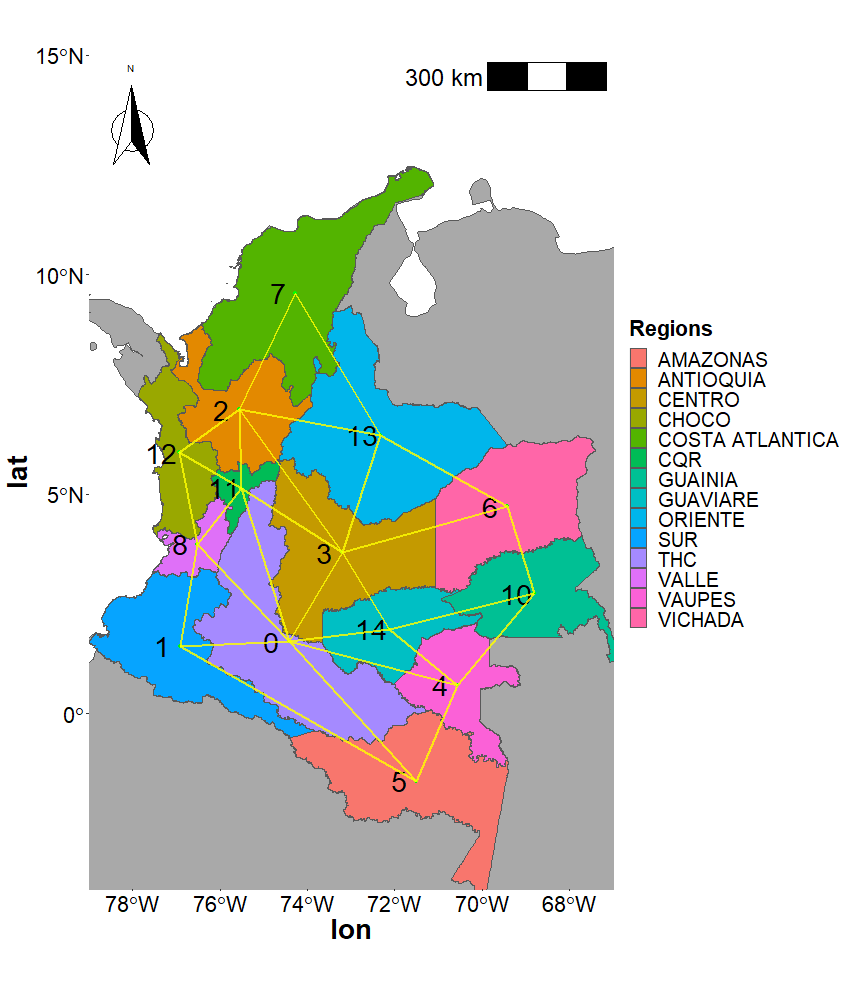
\includegraphics[height=9cm, width=8cm]{figs/Map_Neighborhood_Structure.png}
   \centering
	\caption{\hl{Map} %MDPI: Please consider replacing with a sharper image. %Lina: I can not replace it with a sharper image instead I ajusted the width and height to have a better resolution
	of the neighbourhood structure based on~MRFs.\label{fig:8}}
    \end{figure}
    

    This model can be expressed as Geoadditive regression because it has no further terms but the one with the spatial component such as
\begin{equation}
        g(\mu_i)=R_iv
    \end{equation}
where \(R_i=R[i,s]\) is the incidence matrix between observation i and region  $s$ in which the observation $i$ was collected, and $v$ is the spatially varying effects vector that follows a Gaussian Markov Random Field, GMRF, prior distribution conditional on the variance parameter $\tau^2$ such as \(v_s \vert v_(-s) \sim  \frac{1}{N_s}N\big( 1/N_s \sum_{r \in \delta_s} v_r,\frac{\tau^2}{N_s}\big)\) being $N_s$ the number of neighbours for region s that can also be represented as $\delta_s$ and in this case would represent the neighbourhood relationships shown in Figure~\ref{fig:8}.


    The purely spatial GAM with Markov Random Fields has as a constraint, as it can only be limited to cross-sectional data where the precision penalty matrix $K$ dimensions are based on the set of regions, such as $K$, which has $[s,s]$ dimension. This is why the application of the GMRF in this dataset was limited to aggregated data from one-year---2018.

    \begin{table}[H] 
    \caption{Model summary table for spatial~GAM. \label{tab5}}
    \newcolumntype{C}{>{\centering\arraybackslash}X}
    \begin{tabularx}{\textwidth}{CCCCC}
    \toprule
    \textbf{Rsq} & \textbf{Dev} & \textbf{REML} & \textbf{Scale Est} & \textbf{n}\\
    \midrule
    0.563 & 0.770 & 48.681 & 42.681 & 14\\
    \bottomrule
    \end{tabularx}
    \end{table}
    
    As can be seen in Table~\ref{tab5}, the~resultant spatial model accounts for seventy-seve percent of the electricity demand variation.  The~Akaike Information Criteria AIC for this model is not truly comparable with the non-spatial GAM, which is considerably~higher.

    The was no need to calculate the concurvity, because the model was only dependent on one covariate, which was the Markov Random Fields, and the diagnostic showed that the model converges after five iterations, which means the data is enough for the number of~parameters. 

        \begin{table}[H] 
    \caption{Moran's I test under normality spatial~GAM.\label{tab6}}
    \newcolumntype{C}{>{\centering\arraybackslash}X}
    \begin{tabularx}{\textwidth}{CC}
    \toprule
    \textbf{Moran-I Statistic Stand Deviate} & \textbf{\emph{p}-Value}\\
    \midrule
    0.99897 & 0.15890\\
    \bottomrule
    \end{tabularx}
    \end{table}
\unskip

    \begin{table}[H] 
    \caption{Moran's I test sample estimates of spatial~GAM.\label{tab7}}
    \newcolumntype{C}{>{\centering\arraybackslash}X}
    \begin{tabularx}{\textwidth}{CCC}
    \toprule
    \textbf{Moran-I Statistic} & \textbf{Expectation} & \textbf{Variance}\\
    \midrule
    0.06986 & $-$0.07692 & 0.02158\\
    \bottomrule
    \end{tabularx}
    \end{table}
\unskip
    
    Moran’s I test was calculated to test the spatial autocorrelation in the data, and, as can be seen in Tables~\ref{tab6} and~\ref{tab7} the value obtained showed no autocorrelation meaning the assumption of independence was maintained.
    
    \subsection{Extension of the Non-Spatial GAM with a Spatial-Categorical Regional~Component}
    
    After running both temporal and spatial models as separate. A~final model was built, where a covariate accounting for the regions was included over the already tested temporal one. Unfortunately, there was no way of doing this with Markov Random Fields across longitudinal data.For~this reason, it was decided to use a categorical variable that had the ID of the~regions such as
    
\begin{equation}\label{eq:28}
    \begin{split}
        g(\mu_i)=A_i+f_1^s(hour)+weekday+f_3^T(time)\\+f_{1,2}^I(hour by weekday)+f_{1,3}^I(hour,time)+ID^{spatial}
    \end{split}
    \end{equation}
    
    The components remain the same as the ones in Equation~(\ref{eq:28}) for the non-spatial GAM with the addition of the categorical component that accounts for the IDs of the regions. The~link function keeps being Gaussian, therefore \(d_i \sim N(\mu_i,\phi)\) is~maintained.

    \begin{table}[H] 
    \caption{Model summary table extended non-spatial GAM with a spatial~covariate.\label{tab8}}
    \newcolumntype{C}{>{\centering\arraybackslash}X}
    \begin{tabularx}{\textwidth}{CCCCC}
    \toprule
    \textbf{Rsq} & \textbf{Dev} & \textbf{\hl{REML} %MDPI: Please use scientific notations (e.g., "$8 \times 10^{3}$", not "8E3"). %Lina: Tabled was aligned with text. Scientific notation was corrected.
}  & \textbf{\hl{Scale Est}} & \textbf{n}\\
    \midrule
    0.962 & 0.962 & $6.9594 \times 10^{6}$ & $1.8572 \times 10^{10}$ & 525560\\
    \bottomrule
    \end{tabularx}
    \end{table}

    As can be seen in \hl{Table}%MDPI: Tables 10 and 11 have to be mentioned before Table 12. Please revise. %Lina: Table was moved 
    ~\ref{tab8}, the~resultant extended non-spatial model with the spatial categorical ID variable accounts for ninety-six percent of the electricity demand variation, which is ten percent more than the temporal model by~itself.  

    \begin{table}[H] 
    \caption{Parametric coefficients extended non-spatial GAM with a spatial~covariate.\label{tab9}}
    \newcolumntype{C}{>{\centering\arraybackslash}X}
    \begin{tabularx}{\textwidth}{CCCCC}
    \toprule
    \textbf{Var} & \textbf{Estimate} & \textbf{Std. Error}  & \textbf{\emph{t}-Value} & \textbf{\hl{Pr} %MDPI: Please use scientific notations (e.g., "$8 \times 10^{3}$", not "8E3"). We corrected them. Please confirm.
}\\
    \midrule
    Intercept & 312680.9 & 619.1 & 505.028 & $<2 \times 10^{-16}$\\
    wk/wknd & $-$70008.7 & 416.6 & $-$168.053 & $<2 \times 10^{-16}$\\
    ID1 & $-$88951.4 & 840.8 & $-$105.791 & $<2 \times 10^{-16}$\\
    ID2 & 745127.5 & 882.2 & 844.602 & $<2 \times 10^{-16}$\\
    ID3 & 1809891.3 & 875.7 & 2066.692 &  $<2 \times 10^{-16}$\\
    ID7 & 1407854.7 & 863.1 & 1631.194 & $<2 \times 10^{-16}$\\
    ID8 & 221853.2 & 840.8 & 263.846 & $<2 \times 10^{-16}$\\
    ID11 & 2565.2 & 857.0 & 2.993 & 0.00276\\
    ID12 & $-$262552.1 & 869.4 & $-$301.993 & $<2 \times 10^{-16}$\\
    ID13 & 457133.2 & 844.0 & 541.619 & $<2 \times 10^{-16}$\\
    ID14 & $-$289039.5 & 848.3 & $-$340.734 & $<2 \times 10^{-16}$\\
    \bottomrule
    \end{tabularx}
    \end{table}
\unskip

    \begin{table}[H] 
    \caption{Smooth terms/non-parametric coefficients extended non-spatial GAM with a spatial~covariate.\label{tab10}}
    \newcolumntype{C}{>{\centering\arraybackslash}X}
    \begin{tabularx}{\textwidth}{CCCCC}
    \toprule
    \textbf{Var} & \textbf{Estimate} & \textbf{Std. Error}  & \textbf{\emph{t-}Value} & \textbf{\hl{Pr} %MDPI: Please use scientific notations (e.g., "$8 \times 10^{3}$", not "8E3"). We corrected them. Please confirm.
}\\
    \midrule
    s(hr) & 20.937 & 22 & 24.376 & $<2 \times 10^{-16}$\\
    s(hr):wk/wk & 17.119 & 22 & 4.751 & $<2 \times 10^{-16}$\\
    s(hr):wk/wknd & 2.450 & 22 & 0.120 & $8.57 \times 10^{-15}$\\
    s(time) & 8.989 & 9 & 2723.631 & $<2 \times 10^{-16}$\\
    ti(hr,time) & 126.624 & 198 & 69.221 & $<2 \times 10^{-16}$\\
    \bottomrule
    \end{tabularx}
    \end{table}
\unskip

    
    The Wald t-test from the summary in Tables~\ref{tab9} and~\ref{tab10} for the extended model shows that all smooth terms and parametric terms are highly~significant.

%Lina's changes: Changing numbers for words - Removing overall magnitude and leaving only comparison

    The Akaike Information Criteria AIC for this model was nine times higher than the non-spatial GAM which points to the non-spatial model being a better fit even when the extended model explains more of the demand~variation.

    \begin{table}[H] 
    \caption{K-check extended non-spatial GAM with a spatial~covariate.\label{tab11}}
    \newcolumntype{C}{>{\centering\arraybackslash}X}
    \begin{tabularx}{\textwidth}{CCCCC}
    \toprule
    \textbf{Var} & \textbf{k} & \textbf{edf}  & \textbf{\emph{k}-Index} & \textbf{\emph{p}-Value}\\
    \midrule
    s(hr) & 22 & 21.2287 & 0.9827 & 0.1175\\
    s(hr):wk/wk & 22 & 18.5861 & 0.9827 & 0.1075\\
    s(hr):wk/wknd & 22 & 0.6318 & 0.9827 & 0.1050\\
    s(time) & 9 & 8.8768 & 0.8344 & 0.0000\\
    ti(hr,time) & 198 & 90.1124 & 0.8369 & 0.0000\\
    \bottomrule
    \end{tabularx}
    \end{table}
    
    The model converges after seven iterations, showing the data being enough for the number of parameters, even where the heteroscedasticity still persists for the time individual covariate and its respective interaction as shown in Table~\ref{tab11}.

    %Lina's changes: Phrase was split in two.
    Regarding concurvity, the~conclusions from the non-spatial model are maintained. There concurvity of minor magnitude between the individual effects and the interactions.

           \begin{figure}[H]
	%\centering
		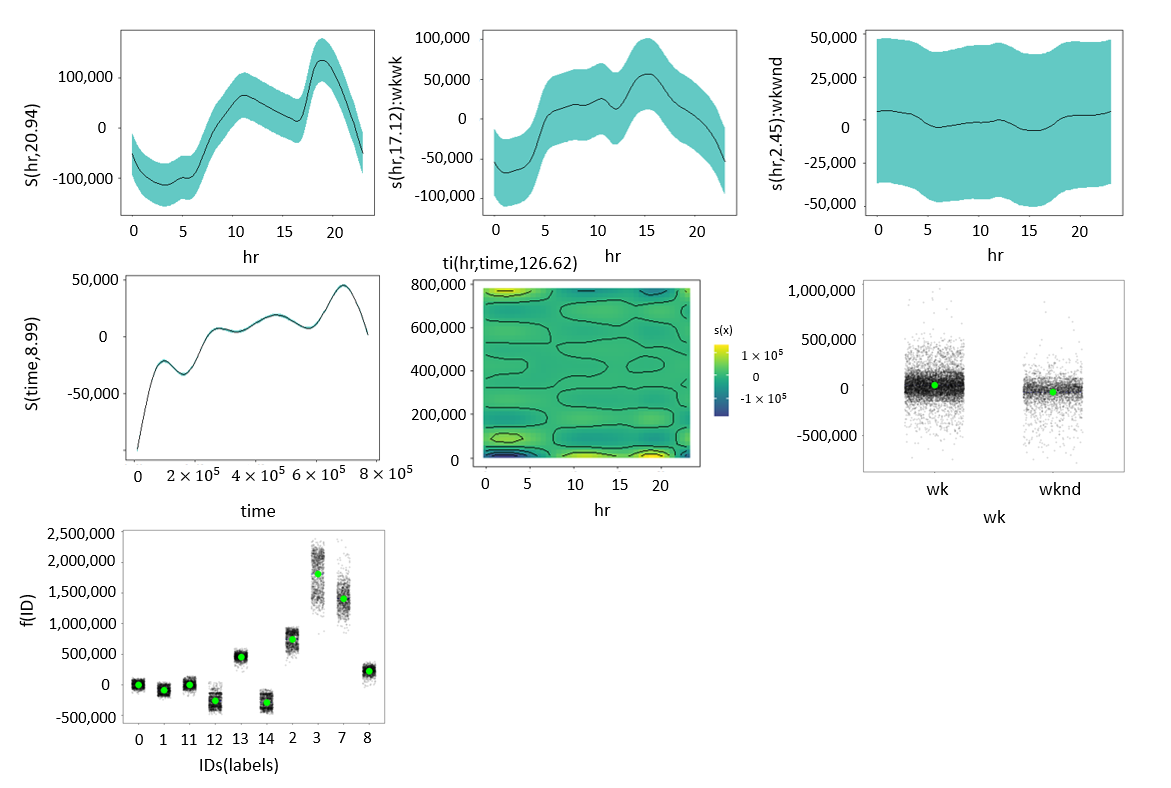
\includegraphics[height=9cm, width=14.5cm]{figs/Partial_Effects_Plot_Extended.png}
	\caption{\hl{Partial} %MDPI: Please consider replacing with a sharper image. % Lina: I changed the resolution I can not replaced it with a density plot because the density covers the shape of the splines
effects for the extended non-spatial GAM with a spatial categorical variable: effects for individual covariates, interaction covariates and parametric factor~terms.	\label{fig:9}}
    \end{figure}
    
    For the extended model the conclusions remain the same as for the non-spatial GAM (See Figure \ref{fig:9}). In this model there is additional information about regions not included in the non-spatial GAM. The model shows predominance in the energy consumption of regions three-Centro, seven-CostaAtlantica, and two-Antioquia when compared against other regions.

   For~the purpose of comparing both models, the~non-spatial GAM without the ID variable was fitted again over the same dataset as the one used for the extended version, so we could run an added variable test to check if the extra variable was contributing to explain the response or~not.
    
    The results in Table~\ref{tab12} show that there is strong evidence that the spatial categorical variable does contribute to explaining the response even when an AIC test between the two models prefers the model with fewer terms. 
    
      \begin{table}[H] 
    \caption{Analysis of deviance~table. \label{tab12}}
    \newcolumntype{C}{>{\centering\arraybackslash}X}
    \begin{tabularx}{\textwidth}{CCCCCC}
    \toprule
    \textbf{Resid. Df} & \textbf{\hl{Resid. Dev} %MDPI: Please use scientific notations (e.g., "$8 \times 10^{3}$", not "8E3").
} & \textbf{Df}  & \textbf{\hl{Deviance}} & \textbf{F} & \textbf{\hl{Pr (>F)}}\\
    \midrule
    525,450
 & $2.3855e+17$ \\
    525,342 & $9.7571e+15$ & 108.3 & $2.2879 \times 10^{17}$ & 113,757 & $<2.2 \times {-16}$\\
    \bottomrule
    \end{tabularx}
    \end{table}

% Lina: Added as a reference of the packages used in R analysis

    \hl{All analyses were performed using R Statistical Software (v4.0.3; R Core Team 2020) } \citep{RCore}.Generalized Additive models were fitted using the mgcv R package (v1.8-33; Wood 2020) \citep{WoodGamDocumentation}. Splines were outlined using the mgcViz R package (v0.1.6; Fasiolo 2020) \citep{mgcVizDocumentation}. Pairwise concurvity was portraited with a heatmap using base R. Maps were elaborated with the ggplot R package(v3.3.2; Wickham 2020) using geometries from the special features sf R package (v0.9.6; Pebesma 2020).

    \clearpage

%Lina's changes: I removed the boxplot it causes confusion when there was already a conclusion of which model explained better the data. There is no need to add information about dispersion.

%%%%%%%%%%%%%%%%%%%%%%%%%%%%%%%%%%%%%%%%%%
\section{Discussion}

%Lina's changes: space and time data --> spatial/temporal data
%Lina's changes: Overall change in the structure of the discussion so it flow better
%Lina's changes: Paragraph about the temporal covariates was removed. It was repeating was it was already stated in the results section.

A holistic approach between spatial/temporal data is hard to accomplish when modelling data with Generalized Additive Models over areas instead of points (discrete-data versus continuous-data). The~fact that data is limited to areas in these case regions makes it difficult to incorporate in longitudinal datasets due to methodologies that model area data across space, such as the two-dimensional smoother Markov Random Fields, are mainly designed for cross-sectional data rather than~longitudinal.

Thin-Plate Spline modelling was considered as another two-dimensional smoothing methodology but was left out of scope due to data needed to be converted from areas into points using centroids. %please verify %Lina: Wording was changed
 In the cases of Colombian regions, such centroids would be more than 100~km away from each other, which would lead to Thin-Plate splines not behaving as a surface but as disaggregated~ellipsoids. %please verify

Due to the previously mentioned limitations of working with areal data, it was decided to first model the individual region’s IDs against the demand and verify the assumptions of spatial autocorrelation with Markov Random Fields. Then the spatial component was incorporated into a temporal extended model using a categorical parameter based on the IDs of the~regions.

Areal data has limitations when visualizing the variation of the dependent variable as a function of the distance using methods such as variograms. Variograms do not work well for areal data, especially when the number of regions is not significant due to there are not enough points to conclude over the pattern and the fact of whether the data is spatially autocorrelated or not. %please verify %Lina: Changed
 Nonetheless, Moran’s I test seems to work equally well for checking the independence, spatial autocorrelation assumptions, regardless of the nature of the data, areal or point-based. %please verify % Lina: Changed

Areal data from wider geographical units such as regions, states, or departments do not allow for the inclusion of a space component as a non-parametric two-dimensional smoother but smaller geographical units like census units, cities, or~households could potentially allow so. While household energy information has identification constraints around it. Aggregation by smaller census areas does not. Energy modelling using household information could lead to more accurate spatial modelling when used in association with population characteristics helping to drive scientific policy advice for the energy~sector.

Heteroscedasticity was found to mainly be connected to the number of knots of the time variable, as shown by the k-test. Increasing the number of knots to get rid of heteroscedasticity was considered but let out of scope to avoid overfitting.

\clearpage


%%%%%%%%%%%%%%%%%%%%%%%%%%%%%%%%%%%%%%%%%%
\section{Conclusions}

% Lina's changes: Changed numbers to words according to APA rules.
% Lina's changes: Adjusted the flow so it reads better
% Lina's changes: Added a last paragraph to mention how does impact policy to link it with the abstract
% Lina's changes: in regards to space and time --> across space and time
% Lina's changes: Complete --> Holistic
% Lina's changes: Nevertheless --> However
% Lina's changes: Accomplish --> Acquire

In this article, the~use of Generalized Additive Models with one-dimensional and two-dimensional smoothers is proposed as an alternative to understand how the energy demand behaves across space and time. A~model using isolated temporal covariates could not be as insightful as one where both time and space aspects are incorporated and would also not be making the most of the GAM features of including multi-dimensional smoothers. The~practical applicability of Markov Random Fields is limited to cross-sectional data when no temporal covariates are included.In~this case, regional IDs in MRFs explain up to seventy-seven percent of the response variation.

The holistic consideration of both space and time leads to the best prediction accuracy, ninety-six percent versus eighty-five percent, from the purely temporal model, but~in this case it is limited to include the regional component as a categorical parameter. In~order to be able to work out the inclusion of a space component as a nonparametric two-dimensional smoother rather than a parametric one, the underlying data would have to come as coordinates and preferably disaggregated to smaller geographical units. However, this level of detail, which may be common in developed countries, it is hard to acquire in developing ones.

Future work as stated in the discussion session would encompass the gathering of point-based information about around energy consumption in the country to validate conclusions obtained with areal data. Minor scale exercises with point-based data in a city or small geographical area will be sufficient to show how a national exercise could be carried and the benefits of point-based data over areal~data.

Availability of point-based data would further enhance the reliability of energy modelling as policy advice.

%%%%%%%%%%%%%%%%%%%%%%%%%%%%%%%%%%%%%%%%%%
\vspace{6pt} 

%%%%%%%%%%%%%%%%%%%%%%%%%%%%%%%%%%%%%%%%%%
%% optional
%\supplementary{The following supporting information can be downloaded at:  \linksupplementary{s1}, Figure S1: title; Table S1: title; Video S1: title.}

% Only for the journal Methods and Protocols:
% If you wish to submit a video article, please do so with any other supplementary material.
% \supplementary{The following supporting information can be downloaded at: \linksupplementary{s1}, Figure S1: title; Table S1: title; Video S1: title. A supporting video article is available at doi: link.}

%%%%%%%%%%%%%%%%%%%%%%%%%%%%%%%%%%%%%%%%%%
 \supplementary{\hl { } %MDPI: Please check if there is supplementary materials of this manuscript. If so, please add the citation in the main text and upload it to the submitting system.
} %Lina: There are no supplemenatary materials

\authorcontributions{\hl{All} %MDPI: For research articles with several authors, a short paragraph specifying their individual contributions must be provided. The following statements should be used ``Conceptualization, X.X. and Y.Y.; methodology, X.X.; software, X.X.; validation, X.X., Y.Y. and Z.Z.; formal analysis, X.X.; investigation, X.X.; resources, X.X.; data curation, X.X.; writing---original draft preparation, X.X.; writing---review and editing, X.X.; visualization, X.X.; supervision, X.X.; project administration, X.X.; funding acquisition, Y.Y. All authors have read and agreed to the published version of the manuscript.'', please turn to the  \href{http://img.mdpi.org/data/contributor-role-instruction.pdf}{CRediT taxonomy} for the term explanation. Authorship must be limited to those who have contributed substantially to the work~reported.
authors have read and agreed to the published version of the~manuscript.} %Lina: This article was produced as a dissertation for a Master of Science from Auckland university. All materials were produced by Lina Berbesi under the supervision of Geoffrey Pritchard.

\funding{This research received no external~funding.}

\informedconsent{Not applicable.}

\dataavailability{Energy demand from Colombia was taken from the publicly archived datasets  from XM ,the entity that oversees the grid of the electricity sector in Colombia. These datasets can be found in the following url \url{https://www.xm.com.co/portal-de-indicadores} \hl{under} %MDPI: Please add the accessed date in the following format: DD Month YYYY.
'regions demand'. Accessed date: 1st January 2019} 

\conflictsofinterest{The authors declare no conflict of~interest.} 

%% Only for journal Encyclopedia
%\entrylink{The Link to this entry published on the encyclopedia platform.}

\abbreviations{Abbreviations}{
The following abbreviations are used in this manuscript:\\

\noindent 
\begin{tabular}{@{}ll}
GAM & Generalized Additive Models\\
GLM & Generalized Linear Models\\
MRF & Markov Random Fields\\
GMRF & Gaussian Markov Random Fields
\end{tabular}
}
%\newpage
%%%%%%%%%%%%%%%%%%%%%%%%%%%%%%%%%%%%%%%%%%
%% Optional
\appendixtitles{no} % Leave argument "no" if all appendix headings stay EMPTY (then no dot is printed after "Appendix A"). If~the appendix sections contain a heading then change the argument to "yes".
\appendixstart
\appendix
\section[\appendixname~\thesection]{}

\begin{table}[H] 
\caption{Grouping of states into~regions.\label{tab15}}
\newcolumntype{C}{>{\centering\arraybackslash}X}
\begin{tabularx}{\textwidth}{CC}
\toprule
\textbf{Region}	& \textbf{State}\\
\midrule
Costa Atlantica		& La~Guajira \\
	         	& Magdalena  \\
           	  & Atlántico  \\
                    & Cesar      \\
                    & Bolívar    \\
                    & Sucre      \\
                    & Córdoba    \\
\midrule
Oriente     		& Norte de~Santander \\
	         	& Santander  \\
           	  & Boyacá     \\
                    & Arauca     \\
                    & Casanare   \\
\midrule
Antioquia     		& Antioquia  \\
\midrule
Chocó     		    & Chocó      \\
\midrule
CQR         		& Caldas     \\
	         	& Risaralda  \\
           	  & Quindío    \\
\midrule
Valle     		    & Valle del~Cauca\\
\midrule
Sur          		& Cauca      \\
	         	& Nariño     \\
           	  & Putumayo   \\
\midrule
Centro          	& Cundinamarca \\
	         	& Bogotá     \\
           	  & Meta       \\
\midrule
Guaviare     	    & Guaviare   \\
\midrule
THC             	& Tolima    \\
	         	& Huila      \\
           	  & Caquetá    \\
\midrule
Amazonas     	    & Amazonas   \\
\midrule
Vaupés     	        & Vaupés     \\
\midrule
Guainía     	    & Guainía     \\
\midrule
Vichada     	    & Vichada     \\
\bottomrule
\end{tabularx}
\end{table}

%Lina's changes: I split the sentences and rephrased the part of how far away it is

The State of San Andres Island was excluded from the regions due to it having its own supply of energy not connected to the national grid, but also due to the fact that the neighbourhood matrix used to capture spatial autocorrelation is based on adjacency. A~distance based neighbourhood matrix could be calculated using K nearest points, or the Euclidean distance. However, San Andres is a disputed island between Nicaragua and Colombia which is closer to mainland Nicaragua (200~km) than to Colombia (700~km) which would cause an unusual neighborhood structure. Distances between the centroids of regions on mainland do not exceed 400km on average. Including San Andres would introduce and outlier in the distance matrix that would later on have to be removed to avoid distortion in the statistical analysis and measurement errors. \clearpage

%\newpage 

%%%%%%%%%%%%%%%%%%%%%%%%%%%%%%%%%%%%%%%%%%
\begin{adjustwidth}{-\extralength}{0cm}
%\printendnotes[custom] % Un-comment to print a list of endnotes

\reftitle{References}

% Please provide either the correct journal abbreviation (e.g., according to the “List of Title Word Abbreviations” http://www.issn.org/services/online-services/access-to-the-ltwa/) or the full name of the journal.
% Citations and References in Supplementary files are permitted provided that they also appear in the reference list here. 

%=====================================
% References, variant A: external bibliography
%=====================================
%\bibliography{your_external_BibTeX_file}

%=====================================
% References, variant B: internal bibliography
%=====================================

%% Loading bibliography style file

% Loading bibliography database
%\bibliography{ref-mendeley-2}


% If authors have biography, please use the format below
%\section*{Short Biography of Authors}
%\bio
%{\raisebox{-0.35cm}{\includegraphics[width=3.5cm,height=5.3cm,clip,keepaspectratio]{Definitions/author1.pdf}}}
%{\textbf{Firstname Lastname} Biography of first author}
%
%\bio
%{\raisebox{-0.35cm}{\includegraphics[width=3.5cm,height=5.3cm,clip,keepaspectratio]{Definitions/author2.jpg}}}
%{\textbf{Firstname Lastname} Biography of second author}

% For the MDPI journals use author-date citation, please follow the formatting guidelines on http://www.mdpi.com/authors/references
% To cite two works by the same author: \citeauthor{ref-journal-1a} (\citeyear{ref-journal-1a}, \citeyear{ref-journal-1b}). This produces: Whittaker (1967, 1975)
% To cite two works by the same author with specific pages: \citeauthor{ref-journal-3a} (\citeyear{ref-journal-3a}, p. 328; \citeyear{ref-journal-3b}, p.475). This produces: Wong (1999, p. 328; 2000, p. 475)

%%%%%%%%%%%%%%%%%%%%%%%%%%%%%%%%%%%%%%%%%%
%% for journal Sci
%\reviewreports{\\
%Reviewer 1 comments and authors’ response\\
%Reviewer 2 comments and authors’ response\\
%Reviewer 3 comments and authors’ response
%}
%%%%%%%%%%%%%%%%%%%%%%%%%%%%%%%%%%%%%%%%%%
\begin{thebibliography}{999}

\bibitem[{United Nations}(2018)]{UnitedNations2018AFFORDABLEEfficient}
{United Nations}.
\newblock {Affordable and Clean Energy: Energy Efficient}. In
\newblock {\em The Sustainable Development Goals Report}; United Nations: {New York, NY, USA}
, 2018.

\bibitem[Bustos~Gonz{\'{a}}lez \em{et~al.}(2014)Bustos~Gonz{\'{a}}lez,
  Sep{\'{u}}lveda, and Aponte]{BustosGonzalez2014NonPerspectives}
Bustos~Gonz{\'{a}}lez, J.F.; Sep{\'{u}}lveda, A.L.; Aponte, K.T.
\newblock {\emph{Zonas no interconectadas eléctricamente en Colombia: problemas y perspectiva (Non Electric Interconnection Zones in Colombia: Problems and Perspectives)}};
\newblock Technical Report;  SSR: {Bogota,Colombia}, \hl{2014}%MDPI: Please add the publisher and the location
.

\bibitem[{WHO}(2009)]{WHO2009TheCountries}
{WHO}.
\newblock {\emph{The Energy Access Situation in Developing Countries}};
\newblock UNDP WHO: New York, NY, USA, 2009; 142p.

\bibitem[Meier \em{et~al.}(2019)Meier, Schneider, and
  Le]{Meier2019Short-termModels}
Meier, J.H.; Schneider, S.; Le, C.
\newblock {\emph{Short-Term Electricity Price Forecasting Using Generalized Additive
  Models}};
\newblock Technical Report; CEUR-WS: {Kiel,Germany}  \hl{2019}%MDPI: Please add the publisher and the location
.

\bibitem[Franco \em{et~al.}(2007)Franco, Dyner, and
  Hoyos]{Franco2007ContributionSouthwest}
Franco, C.; Dyner, I.; Hoyos, S.
\newblock {Contribution of the energy at development of isolated communities in
  not interconnected zones: A case of application of systems dynamics and
  sustainable livelihoods in the Colombia Southwest}. {\emph{DYNA} {\bf 2008}, \emph{75}, 199--214}.

\bibitem[{XM}()]{XMHistoricalDemand}(2019, January 1)
{XM}.
\newblock {\hl{Historical Demand}
\newblock {{https://www.xm.com.co/portal-de-indicadores}}%MDPI: Please provide more information about the article type, such as book (please provide the name and location of the publisher); online resource (please provide the URL of the website and the date it was accessed (Date Month Year)); or journal article (please provide the name of the journal, the year and volume in which it was published, and the page number). Please refer to https://www.mdpi.com/authors/references for full reference formatting guides. 
%Lina : Online Resource https://www.xm.com.co/portal-de-indicadores Accessed on the 1st of January of 2019
}.

\bibitem[Amato \em{et~al.}(2020)Amato, Antoniadis, De~Feis, Goude, and
  Lagache]{Amato2020ForecastingComponents}
Amato, U.; Antoniadis, A.; De~Feis, I.; Goude, Y.; Lagache, A.
\newblock {Forecasting high resolution electricity demand data with additive
  models including smooth and jagged components}.
\newblock {\em Int. J. Forecast.} \textbf{2020}, {\emph{37}, 171--185}.
\newblock {{https://doi.org/10.1016/j.ijforecast.2020.\linebreak 04.001}}.

\bibitem[Wood(2017)]{Wood2017GeneralizedR}
\hl{Wood, S.} %MDPI: Please check if this is duplicated with Reference 19. If so, please remove duplicated references and rearrange all the references to appear in numerical order. Please ensure that there are no duplicated references. 
%Lina: This is a different version of Reference 19. They are both the same book. But this is the one that was published in 2017 while the other one is the one that got published in 2006.
\newblock {\em {Generalized Additive Models: An Introduction with R}};  {R Team: Vienna, Austria}, 2017.

\bibitem[Salem~Jornaz(2016)]{SalemJornaz2016ModelingComponents}
Salem~Jornaz, A. Modeling Daily Electricity Load Curve Using Cubic Splines and
  Functional Principal Components. {Master's Thesis, Missouri University of Science and Technology, Rolla, MI, US}A, 2016.

\bibitem[Perperoglou \em{et~al.}(2019)Perperoglou, Sauerbrei, Abrahamowicz, and
  Schmid]{Perperoglou2019AR}
Perperoglou, A.; Sauerbrei, W.; Abrahamowicz, M.; Schmid, M.
\newblock {A review of spline function procedures in R}.
\newblock {\em BMC Med. Res. Methodol.} {\bf 2019}, {\em 19},~46.
\newblock {{https://doi.org/10.1186/s12874-019-0666-3}}.

\bibitem[Hastie and Tibshirani(1999)]{Hastie1999GeneralizedModels}
Hastie, T.; Tibshirani, R.
\newblock {\em {Generalized Additive Models}};  {Taylor \& Francis: Oxfordshire, UK}, 1999.

\bibitem[Christakos(2005)]{Christakos2005RandomSciences}
Christakos, G.
\newblock {\em {Random Field Models in Earth Sciences}};  Elsevier: {Amsterdam, The Netherlands,} 
2005.

\bibitem[Ibe(2013)]{Ibe2013MarkovEdition}
Ibe, O.C.
\newblock {\em {Markov Processes for Stochastic Modeling}}, 2nd ed.;
  Elsevier Inc.: Amsterdam, The Netherlands, 2013; pp.~{1--494}.
\newblock {{https://doi.org/10.1016/C2012-0-06106-6}}.

\bibitem[Haran(2011)]{Haran2011GaussianData}
Haran, M.
\newblock {\emph{Gaussian Random Field Models for Spatial Data}};
\newblock Technical Report; {Taylor \& Francis: Oxfordshire, UK}, 2011.

\bibitem[Rue and Held(2005)]{Rue2005GaussianApplications}
Rue, H.; Held, L.
\newblock {\em {Gaussian Markov Random Fields: Theory and Applications}}; {Taylor \& Francis: Oxfordshire, UK}, 2005.

\bibitem[Stone(1986)]{Stone1986TheModels}
Stone, C.J.
\newblock {The Dimensionality Reduction Principle for Generalized Additive
  Models}. {\emph{Ann. Stat.} \textbf{1986}, \emph{14}, 590--606}.

\bibitem[Nisbet \em{et~al.}(2018)Nisbet, Miner, and
  Yale]{Nisbet2018BasicOverview}
Nisbet, R.; Miner, G.; Yale, K.
\newblock {Basic Algorithms for Data Mining: A Brief Overview}. In {\em
  Handbook of Statistical Analysis and Data Mining Applications}; Elsevier: {Amsterdam, The Netherlands,} 2018; pp.~121--147.
\newblock {{https://doi.org/10.1016/b978-0-12-416632-5.00007-4}}.

\bibitem[Faraway(2006)]{Faraway2006ExtendingModels}
Faraway, J.J.
\newblock {\em {Extending the Linear Model with R : Generalized Linear, Mixed
  Effects and Nonparametric Regression Models}}; {Taylor \& Francis: Oxfordshire, UK}, 2006.

\bibitem[Wood(2006)]{Wood2006GeneralizedR}
Wood, S.
\newblock {\em {Generalized Additive Models an Introduction with R}}; {R Team: Vienna, Austria}, 2006.

\bibitem[Wood()]{WoodGamDocumentation}(2019,January 1)
\hl{Wood}
%MDPI: Please provide more information about the article type, such as book (please provide the name and location of the publisher); online resource (please provide the URL of the website and the date it was accessed (Date Month Year)); or journal article (please provide the name of the journal, the year and volume in which it was published, and the page number). Please refer to https://www.mdpi.com/authors/references for full reference formatting guides.
, S.
\newblock {mgcv package---R Documentation}. 
\newblock {{https://cran.r-project.org/web/packages/mgcv/mgcv.pdf}}
%Lina: The reference is an URL https://cran.r-project.org/web/packages/mgcv/mgcv.pdf It was accessed as well the 1st of January of 2019

\bibitem[Vasdekis and Vlachonikolis(2005)]{Vasdekis2005OnData}
Vasdekis, V.G.; Vlachonikolis, I.G.
\newblock {On the difference between ML and REML estimators in the modelling of
  multivariate longitudinal data}.
\newblock {\em J. Stat. Plan. Inference} {\bf 2005}, {\em
  134},~194--205.
\newblock {{https://doi.org/10.1016/j.jspi.2004.01.020}}.

\bibitem[Wood(2010)]{Wood2010FastGLMs}
Wood, S.
\newblock {\emph{Fast Stable REML and ML Estimation of Semiparametric GLMs}};
\newblock Technical Report; {Wiley: Hoboken, NJ, USA}, 2010.

\bibitem[Fotheringham \em{et~al.}(2002)Fotheringham, Brunsdon, and
  Charlton]{Fotheringham2002GeographicallyRelationships}
Fotheringham, A.S.; Brunsdon, C.; Charlton, M.
\newblock {\em {Geographically Weighted Regression: The Analysis of Spatially
  Varying Relationships}};  {Wiley: Hoboken, NJ, USA}, 2002.

\bibitem[Fahrmeir \em{et~al.}(2004)Fahrmeir, Kneib, and
  Lang]{Fahrmeir2004PENALIZEDPERSPECTIVE}
Fahrmeir, L.; Kneib, T.; Lang, S.
\newblock {Penalized Structured Additive Regression for Space-Time Data: A
  Bayesian Perspective}. \emph{Stat. Sin.} \textbf{2004}, \emph{14}, 731--761.

\bibitem[Hastie and Tibshirani(1993)]{Hastie1993Varying-CoefficientModels}
Hastie, T.; Tibshirani, R.
\newblock {Varying-Coefficient Models}.
\newblock {\em J. R. Stat. Soc. Ser.} {\bf 1993}, {\em 55},~757--779.
\newblock {{https://doi.org/10.1111/\linebreak j.2517-6161.1993.tb01939.x}}.

\bibitem[Kammann and Wand(2003)]{Kammann2003GeoadditiveModels}
Kammann, E.E.; Wand, M.P.
\newblock {Geoadditive models}.
\newblock {\em J. R. Stat. Soc. Ser.} {\bf 2003}, {\em 52},~{1--18}.
\newblock {{https://doi.org/10.1111/1467-9876.00385}}.

\bibitem[Fahrmeir and Kneib(2011)]{Fahrmeir2011BayesianData}
Fahrmeir, L.; Kneib, T.
\newblock {\em {Bayesian Smoothing and Regression for Longitudinal, Spatial and
  Event History Data}}; {Oxford University Press: Oxford, UK}, 2011.

\bibitem[Stock()]{StockWhatRisk}(2019,January 1)
\hl{Stock}%MDPI: Please provide more information about the article type, such as book (please provide the name and location of the publisher); online resource (please provide the URL of the website and the date it was accessed (Date Month Year)); or journal article (please provide the name of the journal, the year and volume in which it was published, and the page number). Please refer to https://www.mdpi.com/authors/references for full reference formatting guides.
, B.
\newblock {What spatial statistical model is best for predicting fisheries
  bycatch risk?}
\newblock Technical Report.
\newblock {{https://brianstock.github.io/pdf/Stock{\_}bycatch{\_}091117.pdf}}
% Lina: Url https://brianstock.github.io/pdf/Stock_bycatch_091117.pdf Accessed the 1st of January of 2019

\bibitem[Faulkner and Minin(2018)]{Faulkner2018LocallyPriors}
Faulkner, J.R.; Minin, V.N.
\newblock {Locally adaptive smoothing with Markov random fields and shrinkage
  priors}.
\newblock {\em Bayesian Anal.} {\bf 2018}, {\em 13},~225--252.
\newblock {{https://doi.org/10.1214/17-BA1050}}.

\bibitem[Held and Saban{\'{e}}s~Bov{\'{e}}(2020)]{Held2020LikelihoodInference}
Held, L.; Saban{\'{e}}s~Bov{\'{e}}, D.
\newblock {\em {Likelihood and Bayesian Inference}}; Statistics for Biology and
  Health; Springer:  {Berlin/Heidelberg, Germany,} 2020.
\newblock {{https://doi.org/10.1007/978-3-662-60792-3}}.

\bibitem[Saveliev \em{et~al.}(2007)Saveliev, Mukharamova, and
  Zuur]{Saveliev2007AnalysisData}
Saveliev, A.A.; Mukharamova, S.S.; Zuur, A.F.
\newblock {Analysis and Modelling of Lattice Data}. In {\em Analysing
  Ecological Data}; Springer: New York, NY, USA, 2007; pp.~321--339.
\newblock {{https://doi.org/10.1007/978-0-387-45972-1{\_}18}}.

\bibitem[Wang and Yue(2014)]{Wang2014SpatialComputations}
{Wang}, X.F.; Yue, Y.R.
\newblock {{Spatial Gaussian Markov Random Fields: Modelling, Applications
  Spatial Gaussian Markov Random Fields: Modelling, Applications and Efficient
  Computations and Efficient Computations}}. \emph{J. Biomet. Biostat.} \textbf{2014}, \emph{5}, 2.
\newblock {{https://doi.org/10.4172/2155-6180.1000e128}}.

\bibitem[Fahrmeir and Lang(2001)]{Fahrmeir2001BayesianPriors}
Fahrmeir, L.; Lang, S.
\newblock {\emph{Bayesian Inference for Generalized Additive Mixed Models Based on
  Markov Random Field Priors}};
\newblock Technical Report~2; {Wiley: Hoboken, NJ, USA}, 2001.

\bibitem[Fahrmeir and Kneib(2009)]{Fahrmeir2009ProprietyEvidence}
Fahrmeir, L.; Kneib, T.
\newblock {Propriety of posteriors in structured additive regression models:
  Theory and empirical evidence}.
\newblock {\em J. Stat. Plan. Inference} {\bf 2009}, {\em
  139},~843--859.
\newblock {{https://doi.org/10.1016/j.jspi.2008.05.036}}.

\bibitem[{R Core Team}(2019)]{RCore}
R Core Team.
\newblock {\hl{R: A Language and Environment for Statistical Computing}}
\newblock {{https://www.R-project.org/}}

\bibitem[Fasiolo()]{mgcVizDocumentation}(2019,January 1)
\hl{Fasiolo}, M.
\newblock {\hl{mgcViz package- R documentation}}
\newblock {{https://cran.r-project.org/web/packages/mgcViz/mgcViz.pdf}}

\end{thebibliography}
\PublishersNote{}
\end{adjustwidth}
\end{document}
